
\chapter{Eksperymenty}\label{ch:experiment}

\section{Pytania eksperymentalne}

Eksperyment został zaprojektowany, aby odpowiedzieć na następujące pytania:
\begin{itemize}
    \item \textbf{Jaki procent modeli stworzonych przez generator  \textit{ZIMPL} kompiluje się poprawnie?}

Badanie zdolności generatora do tworzenia kodu, który spełni podstawowe wymaganie algorytmu rozwiązującego SCIP. Algorytm określa czy dana zmienna jest możliwa do kompilacji, czy nie, nadając status \texttt{VALID} (poprawny) lub \texttt{NOT VALID} (niepoprawny).

    \item \textbf{Jaki jest procent poprawności odpowiedzi generatora na zbiorze testowym?}

 Określenie średniego poziomu poprawności generowanych rozwiązań na pełnym zbiorze testowym. Poprawność odpowiedzi jest mierzona na podstawie pokrycia generowanego kodu z~oczekiwanym wynikiem dla danego zadania.
    
    \item \textbf{Czy opracowany system generuje modele PL z wyższym prawdopodobieństwem niż kontrolny model językowy?}

Porównanie wyników i przy użyciu stworzonego generatora kodu  \textit{ZIMPL} i wyników generowanych przez model na podstawie standardowego, pojedynczego zapytania. Brana pod uwagę jest liczba poprawnie wygenerowanych odpowiedzi za pomocą pojedynczego zapytania w~porównaniu do liczby odpowiedzi stworzonego generatora.
    
    \item \textbf{Jaką poprawę zapewnia zaawansowane generowanie kodu pod względem jakości składni w stosunku do pojedynczego zapytania?}

Ocena jakości składni dla poszczególnych zapytań pod względem poprawnego zdefiniowania odpowiednich elementów generowanego kodu. Ilość ocenianiach elementów zależy od parametryzacji lub jej braku w stworzonym modelu  \textit{ZIMPL}. Oceny są porównywane między podstawowym zapytaniem, a stworzonym generatorem.
    
\end{itemize}

% TP: TODO: tutaj można dopisać parametry, które są stałe w trakcie eksperymentów (temperatura?) oraz inne założenia

\section{Jaki procent modeli stworzonych przez generator  \textit{ZIMPL} kompiluje się poprawnie?}

\begin{table}
\caption{Tabela sprawdzenia poprawności dla całego zbioru testowego.}\label{tab:experiment:compilation}
\centering%
\begin{tabular}{|l|c|c|}
\hline
\textbf{Status} & \textbf{Suma} & \textbf{Procent} \\
\hline
Poprawne & 3787 & 88,07\% \\
\hline
Niepoprawne & 513 & 11,93\% \\
\hline
\textbf{Razem} & \textbf{4300} & \textbf{100\%} \\
\hline
\end{tabular}
\end{table}

% TP: to są tak proste dane, że nie potrzeba wykresu.
%\begin{figure}[H]
%\centering
%\begin{tikzpicture}
%\begin{axis}[
%    ybar,
%    symbolic x coords={Poprawne, Niepoprawne},
%    xtick=data,
%    ylabel={Liczba},
%    nodes near coords,
%    enlarge x limits=1,
%    bar width=15pt,
%    ymin=0,
%    ymax=4200,
%]
%\addplot coordinates {(Poprawne,3787) (Niepoprawne,513)};
%\end{axis}
%\end{tikzpicture}
%\caption{Wykres wyników sprawdzenia poprawności dla całego zbioru testowego.}\label{rys:plama2a}
%\end{figure}

% TP: połączyłem te dwie tabele w jedną z 5 kolumnami i dodatkowym wierszem nagłówka,
\begin{table}
\caption{Tabela sprawdzenia poprawności w rozbiciu na sztywne i parametryzowane modele}\label{tab:experiment:compilation:breakdown}
\centering%
\begin{tabular}{|l|c|c|c|c|}
\hline%
	&\multicolumn{2}{c|}{Wersja sztywna}&\multicolumn{2}{c|}{Wersja parametryzowana}\\
\hline
\textbf{Status} & \textbf{Suma} & \textbf{Procent} & \textbf{Suma} & \textbf{Procent} \\
\hline
Poprawne & 2129 & 93,58\% & 1658 & 81,88\% \\
\hline
Niepoprawne & 146 & 6,42\% & 367 & 18,12\%\\
\hline
\textbf{Razem} & \textbf{2275} & \textbf{100\%} &\textbf{2025} & \textbf{100\%} \\
\hline
\end{tabular}
\end{table}

% TP: to są tak proste dane, że nie potrzeba wykresu.
%\begin{figure}[H]
%\centering
%\begin{tikzpicture}
%\begin{axis}[
%    ybar,
%    symbolic x coords={Poprawne, Niepoprawne},
%    xtick=data,
%    ylabel={Liczba},
%    nodes near coords,
%    enlarge x limits=1,
%    bar width=15pt,
%    ymin=0,
%    ymax=2400,
%]
%\addplot coordinates {(Poprawne,2129) (Niepoprawne,146)};
%\end{axis}
%\end{tikzpicture}
%\caption{Wykres wyników sprawdzenia poprawności dla sztywnych odpowiedzi.}\label{rys:plama2b}
%\end{figure}

%Podobna weryfikacja została przeprowadzona dla części odpowiedzi, stworzonych w formule parametryzowanej:

%\begin{table}
%\caption{Tabela sprawdzenia poprawności dla parametryzowanych odpowiedzi.}\label{tab:tabela3}
%\centering%
%\begin{tabular}{|l|c|c|}
%\hline
%\textbf{Status} & \textbf{Suma} & \textbf{Procent} \\
%\hline
%Poprawne & 1658 & 81,88\% \\
%\hline
%Niepoprawne & 367 & 18,12\% \\
%\hline
%\textbf{Razem} & \textbf{2025} & \textbf{100\%} \\
%\hline
%\end{tabular}
%\end{table}

% TP: to są tak proste dane, że nie potrzeba wykresu.
%\begin{figure}[H]
%\centering
%\begin{tikzpicture}
%\begin{axis}[
%    ybar,
%    symbolic x coords={Poprawne, Niepoprawne},
%    xtick=data,
%    ylabel={Liczba},
%    nodes near coords,
%    enlarge x limits=1,
%    bar width=15pt,
%    ymin=0,
%    ymax=2000,
%]
%\addplot coordinates {(Poprawne,1658) (Niepoprawne,367)};
%\end{axis}
%\end{tikzpicture}
%\caption{Wykres wyników sprawdzenia poprawności dla parametryzowanych odpowiedzi.}\label{rys:plama2c}
%\end{figure}

% TP: Poniżej moja propozycja krótko i na temat:
Kompiluje się 88,07\% wygenerowanych modeli PL, w tym 95,58\% dla wersji sztywnej i 81,88\% dla wersji parametryzowanej. Tabela~\ref{tab:experiment:compilation} prezentuje liczbę i odsetek przykładów ze zbioru testowego, dla których DMJ wygenerował kompilujący i niekompilujący się kod. Tabela~\ref{tab:experiment:compilation:breakdown} zawiera analogiczne dane w~rozbiciu na wersje sztywną i parametryzowaną problemu.

%Do odpowiedzi na to pytanie został wykorzystany zbiór testowy oraz program SCIP sprawdzający możliwość stworzenia rozwiązania dla podanego modelu PL. Program dla rozwiązania nadaje status \texttt{VALID} (poprawny) lub \texttt{NOT VALID} (niepoprawny). Do weryfikacji i udzielenia odpowiedzi na to pytanie należy zliczyć liczbę poprawnie i niepoprawnie zweryfikowanych kodów oraz obliczyć ich procentową wartość.

%Posługując się zbiorem testowym, zweryfikowane zostały odpowiedzi generatora \textit{ZIMPL}, oraz otrzymały konkretne statusy. \textbf{Procentową wartością, jaka została osiągnięta przy sprawdzaniu poprawnej kompilacji to 88.07\%}. Poniżej zostały przedstawione dokładne wyniki.

%Łączne wyniki generatora \textit{ZIMPL} dla całego zbioru testowego:


%Ze względu na różnice w procesie generacji kodu, zależnie od potrzeby parametryzacji lub stworzenia sztywnego (tzw. hardcoded) modelu  \textit{ZIMPL}, wyniki różnią się od siebie, a co za tym idzie, proces tworzenia parametryzowanego kodu wymaga wykorzystania większej liczby zapytań i~struktury o większej złożoności. % TP: TODO <- jakiej struktury?
%W~związku z tym należy uwzględnić również wyniki dla obu wersji wygenerowanych modeli  \textit{ZIMPL}.

%Łączne wyniki generatora  \textit{ZIMPL} dla zbioru testowego posiadającego odpowiedzi dla wyników kodowanych w formule sztywnej:


Opracowany system generuje poprawne modele z prawdopodobieństwem ponad 80\% niezależnie od przyjętej formy wynikowego modelu PL. %Sumaryczne wyniki, niezależnie od różnicy w formule kodu, oferują ponad 80\% skuteczności. 
Test jest istotny, bo pokazuje, że system radzi sobie z formułowaniem możliwych do rozwiązania modeli LP. Zwłaszcza przy modelach LP ze sztywno zapisanym kodem wynikowym, rezultaty pokazują, że generator potrafi w większości wypadków tworzyć prawidłowo składniowe wyniki. % TP: TODO: <- nie jestem przekonany do tego akapitu. W zasadzie powtarza i rozmywa to co zostało powiedziane wczesniej. Takie ogólnikowe stwierdzenia bardziej pasują do dyskusji.

% TP: TODO: Bardzo ważne: wykonajcie proszę analizy statystyczne:
% - estymacja 95% przedziałów ufności dla prawdopodobieństwa zwrócenia poprawnego modelu: slajd 12 stąd https://theta.edu.pl/wp-content/uploads/2014/02/W11EP.pdf - możecie dopisać do tabel wyżej jako $procent \pm połowa szerokości przedziału$
% - test t lub Z na różnice między prawdopodobieństwami zwrócenia poprawnych modeli w wersj sztywnej i parametryzowanej, np. https://pl.wikipedia.org/wiki/Test_dla_proporcji#Test_dla_dwóch_prób_dużych

\section{Jaki jest procent poprawności odpowiedzi generatora na zbiorze testowym?} % TP: <- usuwam słowo średni, bo "średni procent" nie brzmi poprawnie; niżej też

% TP: TODO: Bardzo proszę, przeróbcie ten tekst w stylu poprzedniej sekcji: krótka odpowiedź na pytanie z nagłówka + wyrzucić wykresy + zagregować tabele 5.4 i 5.5  oraz 5.7 i 5.8 + analiza statystyczna.
% Tutaj trzeba jeszcze wyjaśnić jak jest weryfikowana poprawność odpowiedzi, bo z poniższego tekstu to nie wynika. 

Do uzyskania procenta poprawności odpowiedzi, potrzebne są konkretne rezultaty pozyskane z algorytmu rozwiązującego SCIP. Takie wyniki zostały porównane z wynikami poprawnych rozwiązań i na podstawie porównania otrzymywały status poprawnego lub niepoprawnego rozwiązania. Do takiej weryfikacji brane pod uwagę były jedynie rozwiązania, które uzyskały status poprawnego (VALID) podczas poprzedniego eksperymentu.

\textbf{Procent poprawności odpowiedzi względem poprawnych wyników, przeanalizowany na zbiorze testowym, wynosi 60,93\%.} Ten sam wynik analizowany na \textbf{zbiorze testowym wyłączając wyniki, które nie zostały poprawnie skompilowane w poprzednim etapie, procent poprawności wynosi 69,18\%}. Poniżej przedstawiona jest tabela uwzględniająca wszystkie dane testowe wraz z wynikiem analizy rozwiązań.

\begin{table}[ht]
\caption{Tabela sprawdzenia wygenerowanego kodu względem poprawnych wyników dla wszystkich danych testowych.}\label{tab:tabela4}
\centering%
\begin{tabular}{|l|c|c|}
\hline
\textbf{Status} & \textbf{Suma} & \textbf{Procent} \\
\hline
Zgadzające się & 2620 & 60,93\% \\
\hline
Niezgadzające się & 1167 & 27,14\% \\
\hline
Nieuwzględnione & 513 & 11,93\% \\
\hline
\textbf{Razem} & \textbf{4300} & \textbf{100\%} \\
\hline
\end{tabular}
\end{table}

\begin{figure}[H]
\centering
\begin{tikzpicture}
\begin{axis}[
    ybar,
    symbolic x coords={Zgadzające się, Niezgadzające się, Nieuwzględnione},
    xtick=data,
    ylabel={Liczba},
    nodes near coords,
    bar width=15pt,
    ymin=0,
    ymax=2900,
]
\addplot coordinates {(Zgadzające się,2620) (Niezgadzające się,1167) (Nieuwzględnione,513)};
\end{axis}
\end{tikzpicture}
\caption{Wykres wyników sprawdzenia wygenerowanego kodu względem poprawnych wyników dla wszystkich danych testowych.}\label{rys:plama2d}
\end{figure}

Tak jak w pierwszym pytaniu eksperymentalnym, przeprowadzono również analizę ze względu na formułę wygenerowanego kodu. Uwzględniono przy tym procent ominiętych rezultatów. Dla wyników sztywnego kodowania poprawne wartości wynosiły 60\%, podczas gdy dla wyników parametryzowanego kodu wyniosły one 61,98\%. Sumaryczne wyniki prezentują się jak poniżej.

\begin{table}[ht]
\caption{Tabela sprawdzenia wygenerowanego kodu względem poprawnych wyników dla sztywnych odpowiedzi.}\label{tab:tabela5}
\centering%
\begin{tabular}{|l|c|c|}
\hline
\textbf{Status} & \textbf{Suma} & \textbf{Procent} \\
\hline
Zgadzające się & 1365 & 60,00\% \\
\hline
Niezgadzające się & 764 & 33,58\% \\
\hline
Nieuwzględnione & 146 & 6,42\% \\
\hline
\textbf{Razem} & \textbf{2275} & \textbf{100\%} \\
\hline
\end{tabular}
\end{table}

\begin{figure}[H]
\centering
\begin{tikzpicture}
\begin{axis}[
    ybar,
    symbolic x coords={Zgadzające się, Niezgadzające się, Nieuwzględnione},
    xtick=data,
    ylabel={Liczba},
    nodes near coords,
    bar width=15pt,
    ymin=0,
    ymax=1600,
]
\addplot coordinates {(Zgadzające się,1365) (Niezgadzające się,764) (Nieuwzględnione,146)};
\end{axis}
\end{tikzpicture}
\caption{Wykres wyników sprawdzenia wygenerowanych wyników względem poprawnych wyników dla sztywnych odpowiedzi.}\label{rys:plama2e}
\end{figure}

\begin{table}[ht]
\caption{Tabela sprawdzenia wygenerowanych wyników względem poprawnych wyników dla parametryzowanych odpowiedzi.}\label{tab:tabela6}
\centering%
\begin{tabular}{|l|c|c|}
\hline
\textbf{Status} & \textbf{Suma} & \textbf{Procent} \\
\hline
Zgadzające się & 1255 & 61,98\% \\
\hline
Niezgadzające się & 403 & 19,90\% \\
\hline
Nieuwzględnione & 367 & 18,12\% \\
\hline
\textbf{Razem} & \textbf{2025} & \textbf{100\%} \\
\hline
\end{tabular}
\end{table}

\begin{figure}[H]
\centering
\begin{tikzpicture}
\begin{axis}[
    ybar,
    symbolic x coords={Zgadzające się, Niezgadzające się, Nieuwzględnione},
    xtick=data,
    ylabel={Liczba},
    nodes near coords,
    bar width=15pt,
    ymin=0,
    ymax=1500,
]
\addplot coordinates {(Zgadzające się,1255) (Niezgadzające się,403) (Nieuwzględnione,367)};
\end{axis}
\end{tikzpicture}
\caption{Wykres wyników sprawdzenia wygenerowanych wyników względem poprawnych wyników dla parametryzowanych odpowiedzi.}\label{rys:plama2f}
\end{figure}

Dla porównania, taka sama analiza została przeprowadzona dla wszystkich wyników, ale nie uwzględniając wartości, które zostały wykluczone jako niepoprawne, przy odpowiedzi na poprzednie pytanie eksperymentalne. Dzięki temu lepiej widoczne są wyniki poprawności generowanego kodu i podziału ze względu na pokrywające się wyniki. Wnioskiem z tego eksperymentu jest skuteczność w okolicy 70\% dla kodu zweryfikowanego jako możliwy do kompilacji.

\begin{table}[ht]
\caption{Tabela sprawdzenia poprawności dla zbioru testowego oznaczonego jako możliwy do kompilowania.}\label{tab:tabela7}
\centering%
\begin{tabular}{|l|c|c|}
\hline
\textbf{Status} & \textbf{Suma} & \textbf{Procent} \\
\hline
Zgadzające się & 2620 & 69,18\% \\
\hline
Niezgadzające się & 1167 & 30,82\% \\
\hline
\textbf{Razem} & \textbf{3787} & \textbf{100\%} \\
\hline
\end{tabular}
\end{table}

\begin{figure}[H]
\centering
\begin{tikzpicture}
\begin{axis}[
    ybar,
    symbolic x coords={Zgadzające się, Niezgadzające się},
    xtick=data,
    ylabel={Liczba},
    nodes near coords,
    enlarge x limits=0.5,
    bar width=15pt,
    ymin=0,
    ymax=2900,
]
\addplot coordinates {(Zgadzające się,2620) (Niezgadzające się,1167)};
\end{axis}
\end{tikzpicture}
\caption{Wykres wyników sprawdzenia poprawności dla zbioru testowego oznaczonego jako możliwy do kompilowania.}\label{rys:plama2g}
\end{figure}

Podobna weryfikacja możliwa jest dla wyników sformułowanych jako sztywne oraz parametryzowane. W tym przypadku wynik parametryzowanych odpowiedzi jest lepszy od wyniku sztywnego kodowania i wynosi 75,69\%. W związku z tym generator posiada lepszą zdolność do tworzenia kodów możliwych do kompilacji w przypadku sztywnego kodowania, natomiast gdy kod jest poprawnie skompilowany, parametryzowany kod jest częściej tym poprawnym pod względem wyniku.

\begin{table}[ht]
\caption{Tabela sprawdzenia poprawności dla zbioru testowego oznaczonego jako możliwy do kompilowania oraz kodowanego w sposób sztywny.}\label{tab:tabela8}
\centering%
\begin{tabular}{|l|c|c|}
\hline
\textbf{Status} & \textbf{Suma} & \textbf{Procent} \\
\hline
Zgadzające się & 1365 & 64,11\% \\
\hline
Niezgadzające się & 764 & 35,89\% \\
\hline
\textbf{Razem} & \textbf{2129} & \textbf{100\%} \\
\hline
\end{tabular}
\end{table}

\begin{figure}[H]
\centering
\begin{tikzpicture}
\begin{axis}[
    ybar,
    symbolic x coords={Zgadzające się, Niezgadzające się},
    xtick=data,
    ylabel={Liczba},
    nodes near coords,
    enlarge x limits=0.5,
    bar width=15pt,
    ymin=0,
    ymax=1600,
]
\addplot coordinates {(Zgadzające się,1365) (Niezgadzające się,764)};
\end{axis}
\end{tikzpicture}
\caption{Wykres wyników sprawdzenia poprawności dla zbioru testowego oznaczonego jako możliwy do kompilowania oraz kodowanego w sposób sztywny.}\label{rys:plama2h}
\end{figure}

\begin{table}[ht]
\caption{Tabela sprawdzenia poprawności dla zbioru testowego oznaczonego jako możliwy do kompilowania oraz kodowanego w sposób parametryzowany.}\label{tab:tabela9}
\centering%
\begin{tabular}{|l|c|c|}
\hline
\textbf{Status} & \textbf{Suma} & \textbf{Procent} \\
\hline
Zgadzające się & 1255 & 75,69\% \\
\hline
Niezgadzające się & 403 & 24,31\% \\
\hline
\textbf{Razem} & \textbf{1658} & \textbf{100\%} \\
\hline
\end{tabular}
\end{table}

\begin{figure}[H]
\centering
\begin{tikzpicture}
\begin{axis}[
    ybar,
    symbolic x coords={Zgadzające się, Niezgadzające się},
    xtick=data,
    ylabel={Liczba},
    nodes near coords,
    enlarge x limits=0.5,
    bar width=15pt,
    ymin=0,
    ymax=1500,
]
\addplot coordinates {(Zgadzające się,1255) (Niezgadzające się,403)};
\end{axis}
\end{tikzpicture}
\caption{Wykres wyników sprawdzenia poprawności dla zbioru testowego oznaczonego jako możliwy do kompilowania oraz kodowanego w sposób parametryzowany.}\label{rys:plama2i}
\end{figure}

Przy interpretowaniu tych wyników należy uwzględnić czynniki, które mogły powodować szumy. Jednym z nich jest niepoprawna interpretacja zadania przez generator. W przypadku, gdy model językowy zrozumie zadanie w inny sposób niż autor bazy, wynik automatycznie jest klasyfikowany jako niepoprawny, mimo że nie zawsze będzie błędny względem treści zadania.

\section{Czy opracowany system generuje modele PL z wyższym prawdopodobieństwem niż kontrolny model językowy?}
% TP: TODO: Tutaj też sugeruję skrócić odpowiedź i usunąć rysunek 5.7; 5.8 może zostać
% To co nazywacie "pojedynczym zapytaniem" lepiej nazwać "kontrolnym DMJ" i trzeba krótko napisać co to dokładnie jest, tj. GPT-4o-mini?
% Pilnujcie nazewnictwa; nie "rozwiązanie", a "model":

Weryfikacja rozwiązania, poza sprawdzeniem poprawności generowanego kodu, odbywa się również poprzez porównanie jego wyników do wyników standardowego zapytania skierowanego do modelu językowego. Jako standardowe zapytanie rozumiane jest zapytanie w formacie:

\begin{quote}
\begin{verbatim}
<Zapytanie o napisanie kodu  ZIMPL> <zadanie, dla którego oczekiwane jest
roziwązanie>
\end{verbatim}
\end{quote}

Kod generowany poprzez takie zapytanie przechodzi jeszcze obróbce końcowej, w tym usuwaniu zbędnych znaków wywołujących niepotrzebne zakłócenia w interpretacji kodu. % TP: TODO: jakiej konkretnie obróbce? Jakich znaków?
Zdecydowano się na taki krok ze względu na brak skuteczności, % TP: TODO: <- w eksperymentach są pokazywane konkretne miary, więc należy używać ich nazw; "skuteczność" nie jest zdefiniowana
w celu faktycznego sprawdzenia, czy kod jest poprawny, niezależnie od dodatkowych informacji przekazywanych w odpowiedzi.

\textbf{Istnieje znacząca poprawa w jakości wygenerowanego rozwiązania w stosunku do rozwiązania za pomocą pojedynczego zapytania.} Testy poprowadzone na jednorazowym zapytaniu, wykorzystując model językowy GPT-4o-mini oraz temperaturę = 0, czyli dokładnie takie parametry, jakie zostały zastosowane w przypadku stworzonego generatora, jasno wskazują na zerową skuteczność. Rezultaty nigdy nie osiągają statusu poprawnego, a tym samym nie są rozważane przy porównywaniu rozwiązań. DMJ nie zna składni języka  \textit{ZIMPL}, w związku z czym dodaje do niego niepoprawne elementy kodu, zwłaszcza w przypadku deklaracji ograniczeń. Nie jest świadomy wszystkich koniecznych do kompilacji elementów kodu, a także generuje podstawowe błędy przy odczytywaniu wartości z polecenia. Wynik sprawdzania poprawności uwzględnia jedynie sprawdzenie możliwości kompilacji kodu. Nie ma potrzeby przeprowadzania dalszych testów, albowiem musiałyby przebiegać na pustym zbiorze rozwiązań.

\begin{table}[ht]
\caption{Tabela sprawdzenia poprawności dla zbioru testowego przy zastosowaniu pojedynczego zapytania.}\label{tab:tabela10}
\centering%
\begin{tabular}{|l|c|c|}
\hline
\textbf{Status} & \textbf{Suma} & \textbf{Procent} \\
\hline
Poprawne & 0 & 0,00\% \\
\hline
Niepoprawne & 4300 & 100,00\% \\
\hline
\textbf{Razem} & \textbf{4300} & \textbf{100\%} \\
\hline
\end{tabular}
\end{table}

\begin{figure}[H]
\centering
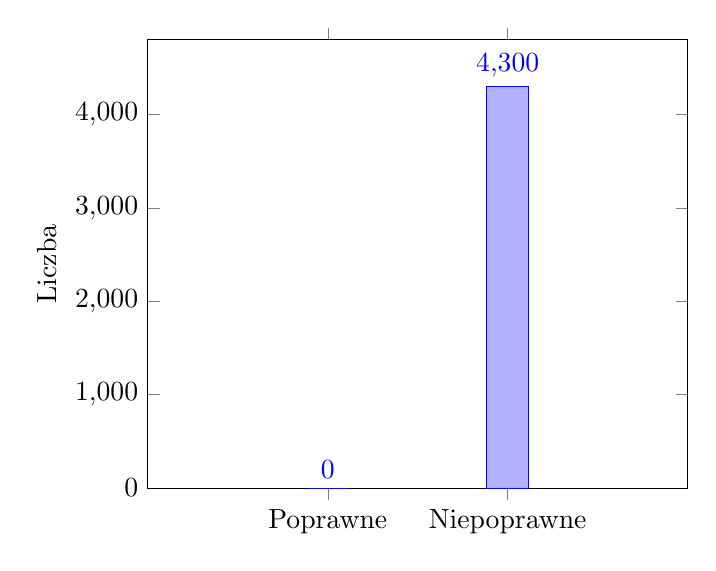
\begin{tikzpicture}
\begin{axis}[
    ybar,
    symbolic x coords={Poprawne, Niepoprawne},
    xtick=data,
    ylabel={Liczba},
    nodes near coords,
    enlarge x limits=1,
    bar width=15pt,
    ymin=0,
    ymax=4800,
]
\addplot coordinates {(Poprawne,0) (Niepoprawne,4300)};
\end{axis}
\end{tikzpicture}
\caption{Wykres wyników sprawdzenia poprawności dla zbioru testowego przy zastosowaniu pojedynczego zapytania.}\label{rys:plama2j}
\end{figure}

Ostateczne zestawienie wyników generatora z jednym zapytaniem w formie tablicy kontyngencji, uwzględniając przy tym weryfikację możliwości kompilacji kodu wygląda w tym przypadku następująco:

\begin{table}[ht]
\caption{Tablica kontyngencji dla zbioru testowego przy zastosowaniu pojedynczego zapytania oraz generatora kodu.}\label{tab:tabela11}
\centering%
\begin{tabular}{|l|l|c|c|}
\hline
\textbf{Generator} & \textbf{Pojedyncze zapytanie} & \textbf{Suma} & \textbf{Procent} \\
\hline
Poprawne & Poprawne & 0 & 0,00\% \\
\hline
Poprawne & Niepoprawne & 3787 & 88,07\% \\
\hline
Niepoprawne & Poprawne & 0 & 0,00\% \\
\hline
Niepoprawne & Niepoprawne & 513 & 11,93\% \\
\hline
\textbf{Razem} & & \textbf{4300} & \textbf{100\%} \\
\hline
\end{tabular}
\end{table}

Dla wykresu zastosowano skrócone nazewnictwo, w którym komplementarnie do powyższej tabeli, prawy znak dotyczy wyników stworzonego generatora podczas gdy lewy znak dotyczy wyników pojedynczego zapytania.

\begin{figure}[H]
\centering
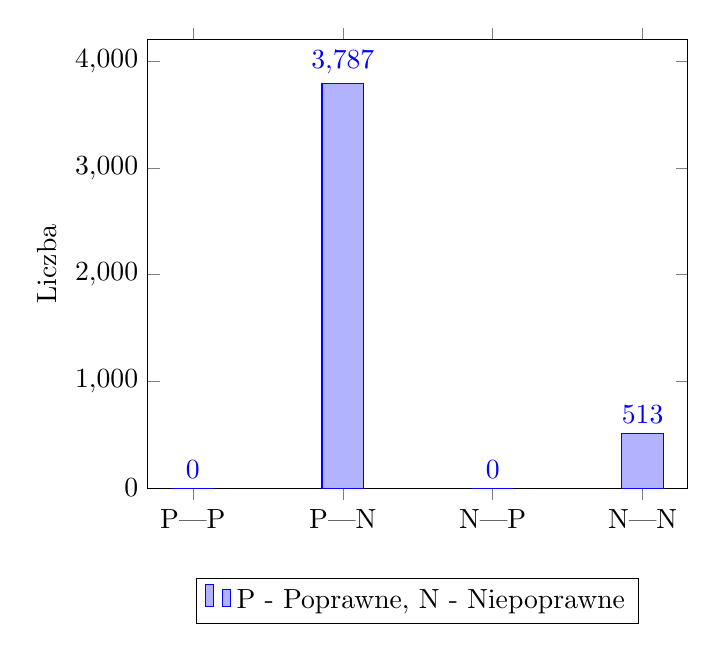
\begin{tikzpicture}
\begin{axis}[
    ybar,
    symbolic x coords={P|P, P|N, N|P, N|N},
    xtick=data,
    ylabel={Liczba},
    nodes near coords,
    bar width=15pt,
    legend style={at={(0.5,-0.20)}, anchor=north, legend columns=-1},
    ymin=0,
    ymax=4200,
]
\addplot coordinates {(P|P,0) (P|N,3787) (N|P,0) (N|N,513)};
\addlegendentry{P - Poprawne, N - Niepoprawne}
\end{axis}
\end{tikzpicture}
\caption{Wykres wyników sprawdzenia poprawności dla zbioru testowego przy zastosowaniu pojedynczego zapytania oraz generatora kodu.}\label{rys:plama2k}
\end{figure}

\section{Jaką poprawę zapewnia zaawansowane generowanie kodu pod względem jakości składni w stosunku do pojedynczego zapytania?}

Do sprawdzenia jakości modelu pod względem jego składni i jakości zrozumienia zadania wykorzystano model GPT-4o. Po otrzymaniu wyników, dla większej wiarygodności, wykonano oczyszczanie rezultatów i naprawę oczywistych błędów halucynowanych przez model. Zależnie od funkcjonalności kodu, wykorzystano inne mierniki jakości. Dla wyników parametryzowanych zastosowano skalę sześciostopniową, podczas gdy dla sztywnego kodowania - czterostopniową.

Wynikiem eksperymentu jest punktacja \textbf{3,31/4,00} dla wygenerowanych wyników, w porównaniu do \textbf{1,81/4,00} dla standardowego zapytania, dla wszystkich wyników sztywnego kodowania. Tak samo, dla parametryzowanych wyników powstałych w wyniku wykorzystania generatora oceną jest \textbf{4,75/6,00}, podczas gdy dla pojedynczego zapytania wynosi \textbf{2,78/6,00}. Sumaryczna poprawa względem standardowego zapytania \textbf{wzrosła o średnio 1,74} punktu.

\subsection{Wyniki dla modelu zapisanego w sztywnej formule.}

Aby poprawnie zweryfikować wyniki, rozpatrzone zostały poszczególne elementy modelu wynikowego. Na początku rozważony zostanie model kodu zapisanego w \textbf{sztywnej formule}. Wszystkie wyniki są porównywane z poprawnym kodem zawartym w danych testowych. W tej skali punktowane były poszczególne elementy:

\begin{enumerate}
\item (1 punkt) \textbf{Definiowanie zmiennych} -- aby uzyskać punkt w tej kategorii, zmienne i typy muszą być zgodne ze sobą. Ich nazwy i komentarze mogą się od siebie różnić, ale logika musi pozostać taka sama. Brak zgodności powoduje utratę punktu.
\item (1 punkt) \textbf{Funkcja celu} -- punkt przyznawany jest za poprawne zdefiniowanie funkcji celu. Musi być zgodna w strukturze, współczynnikach oraz poprawnie zdefiniowana za pomocą uwzględnienia minimalizacji lub maksymalizacji. Brak nazwy lub niezgodna struktura powodują utratę punktu.
\item (1 punkt) \textbf{Ograniczenia} -- aby otrzymać punkt, ograniczenia muszą być zdefiniowane zgodnie z poprawnym kodem. Liczba, logika i zapis muszą być zgodne, a każde ograniczenie powinno zaczynać się od \texttt{subto <nazwa>:}. Zastosowanie innej struktury powoduje odjęcie punktu.
\item (1 punkt) \textbf{Inne wymagania} -- punkt przyznaje się za spełnienie wymagań takich jak: użycie \texttt{\#} jako prefiksu komentarzy, brak zbędnych poleceń oraz poprawne rozpoczęcie każdej linii od jednego z kluczowych słów (\texttt{var}, \texttt{minimize}, \texttt{maximize}, \texttt{subto}).
\end{enumerate}

Poniżej przedstawiona została analiza wyników generatora oraz pojedynczego zapytania dla poszczególnych kategorii.

\begin{table}[ht]
\caption{Tabela ocenionych wyników dla kategorii \textbf{Definiowanie zmiennych}.}\label{tab:tabela12}
\centering%
\begin{tabular}{|l|c|c|}
\hline
\textbf{Punktacja} & \textbf{Generator} & \textbf{Pojedyncze zapytanie}\\
\hline
1 & 1832 & 1418 \\
\hline
0 & 443 & 857 \\
\hline
Średnia ocena & 0,81 & 0,62 \\
\hline
\end{tabular}
\end{table}

\begin{figure}[H]
\centering
\begin{minipage}{0.45\textwidth}
\centering
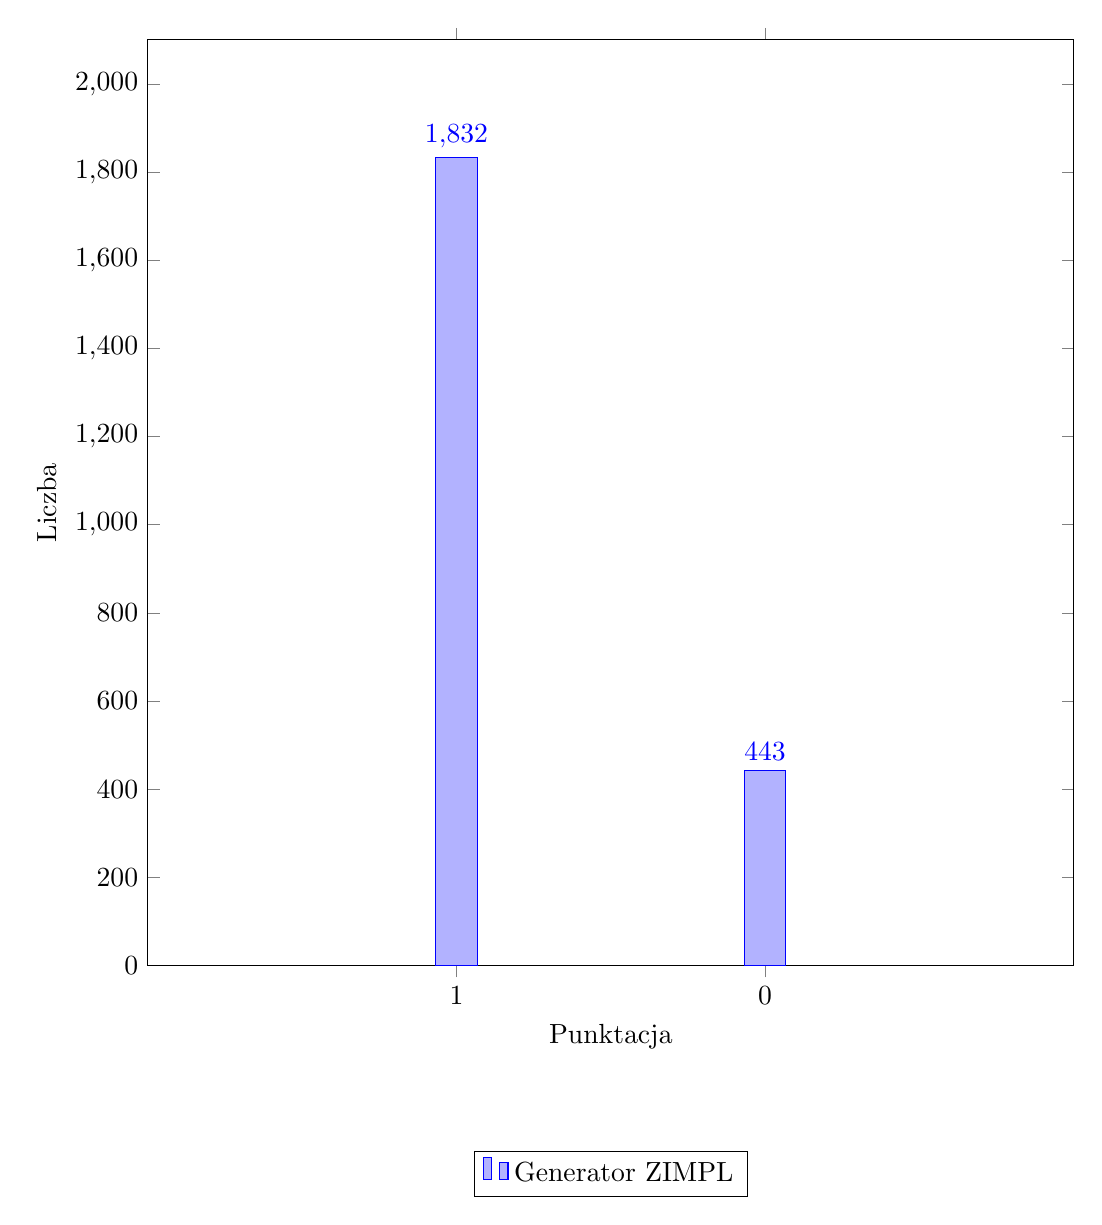
\begin{tikzpicture}
\begin{axis}[
    ybar,
    symbolic x coords={1, 0},
    xtick=data,
    ylabel={Liczba},
    width=1.1\textwidth,
    height=1.1\textwidth,
    nodes near coords,
    bar width=15pt,
    enlarge x limits=1,
    ymin=0,
    ymax=2100,
    xlabel={Punktacja},
    legend style={at={(0.5,-0.20)}, anchor=north, legend columns=-1}
]
\addplot coordinates {(1,1832) (0,443)};
\addlegendentry{Generator ZIMPL}
\end{axis}
\end{tikzpicture}
\end{minipage}%
\hspace{0.05\textwidth}
\begin{minipage}{0.45\textwidth}
\centering
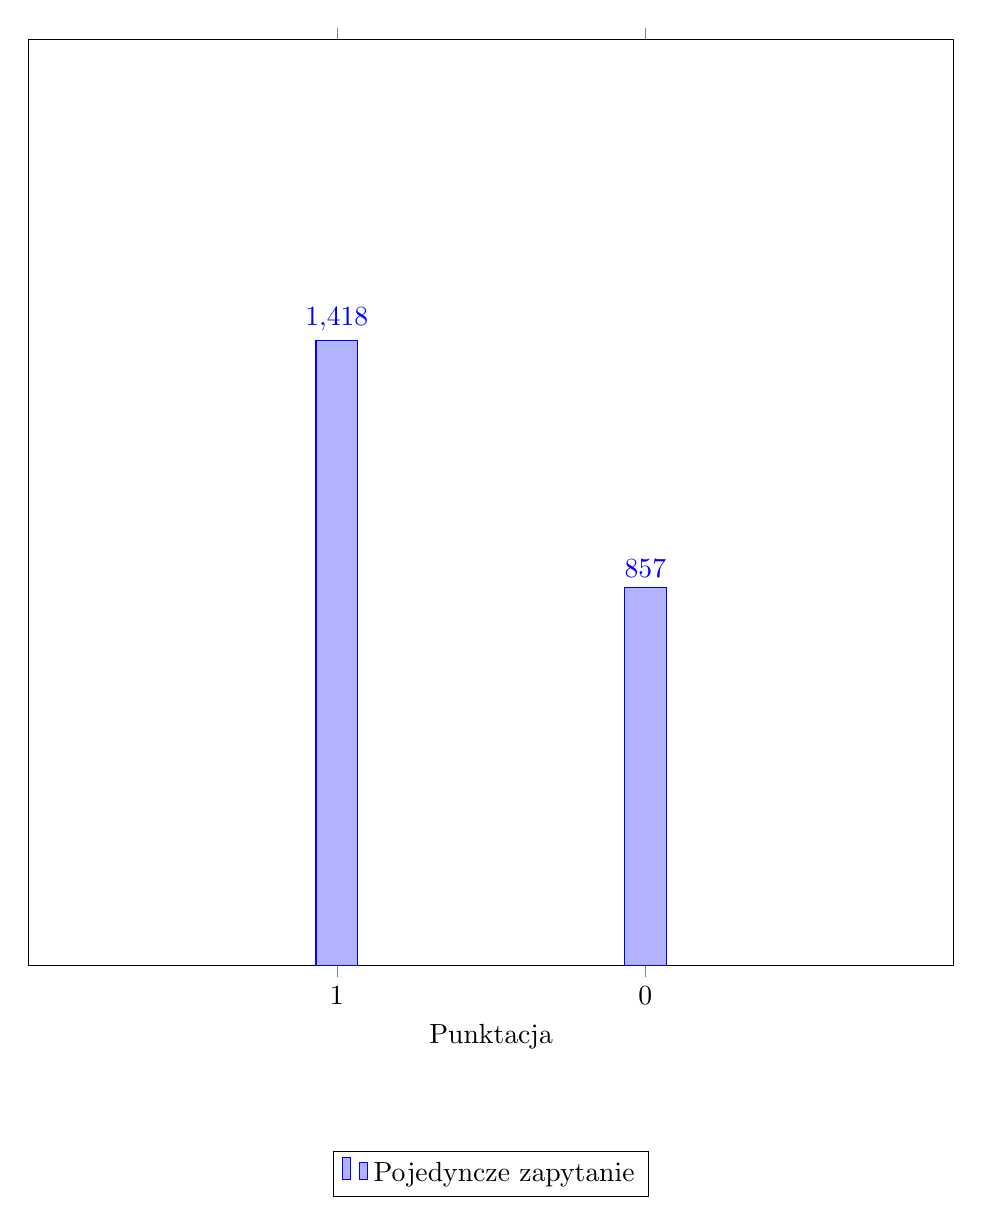
\begin{tikzpicture}
\begin{axis}[
    ybar,
    symbolic x coords={1, 0},
    xtick=data,
    %ylabel={Liczba},
    width=1.1\textwidth,
    height=1.1\textwidth,
    ytick = \empty,
    nodes near coords,
    bar width=15pt,
    enlarge x limits=1,
    ymin=0,
    ymax=2100,
    xlabel={Punktacja},
    legend style={at={(0.5,-0.20)}, anchor=north, legend columns=-1}
]
\addplot coordinates {(1,1418) (0,857)};
\addlegendentry{Pojedyncze zapytanie}
\end{axis}
\end{tikzpicture}
\end{minipage}
\caption{Wykres ocenionych wyników dla kategorii \textbf{Definiowanie zmiennnych}.}
\end{figure}

Już pierwszy wynik pokazuje większą skuteczność generatora ponad pojedynczym zapytaniem. Podstawowym błędem popełnianym w deklaracji zmiennych jest niezgodna w porównaniu z zadaniem ich liczba.

\begin{table}[ht]
\caption{Tabela ocenionych wyników dla kategorii \textbf{Funkcja celu}.}\label{tab:tabela13}
\centering%
\begin{tabular}{|l|c|c|}
\hline
\textbf{Punktacja} & \textbf{Generator} & \textbf{Pojedyncze zapytanie}\\
\hline
1 & 1882 & 1469 \\
\hline
0 & 393 & 806 \\
\hline
Średnia ocena & 0,83 & 0,65 \\
\hline
\end{tabular}
\end{table}

\begin{figure}[H]
\centering
\begin{minipage}{0.45\textwidth}
\centering
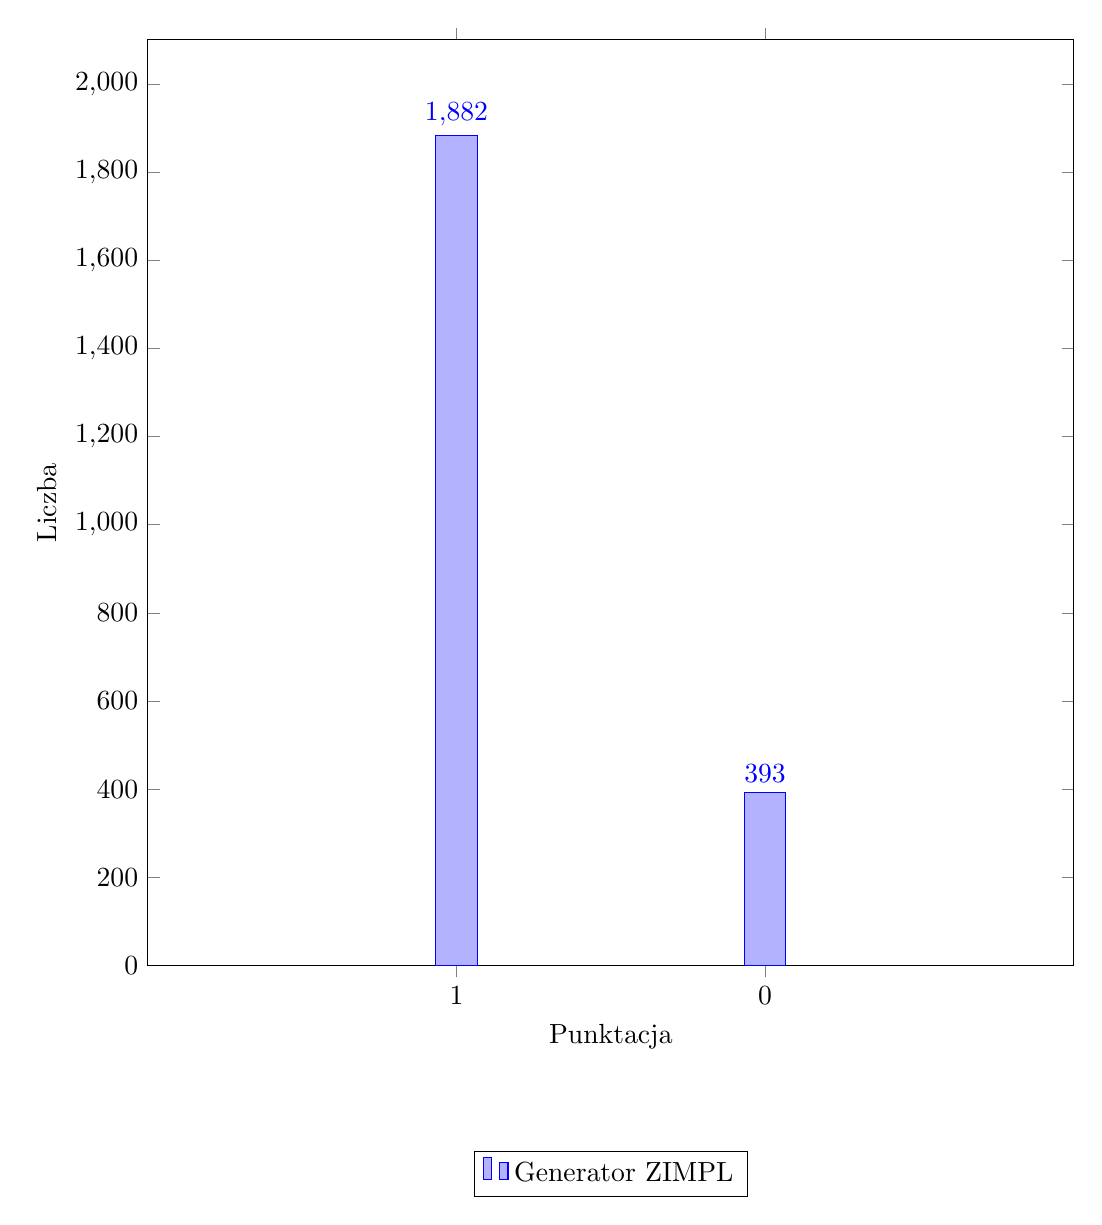
\begin{tikzpicture}
\begin{axis}[
    ybar,
    symbolic x coords={1, 0},
    xtick=data,
    ylabel={Liczba},
    width=1.1\textwidth,
    height=1.1\textwidth,
    nodes near coords,
    bar width=15pt,
    enlarge x limits=1,
    ymin=0,
    ymax=2100,
    xlabel={Punktacja},
    legend style={at={(0.5,-0.20)}, anchor=north, legend columns=-1}
]
\addplot coordinates {(1,1882) (0,393)};
\addlegendentry{Generator ZIMPL}
\end{axis}
\end{tikzpicture}
\end{minipage}%
\hspace{0.05\textwidth}
\begin{minipage}{0.45\textwidth}
\centering
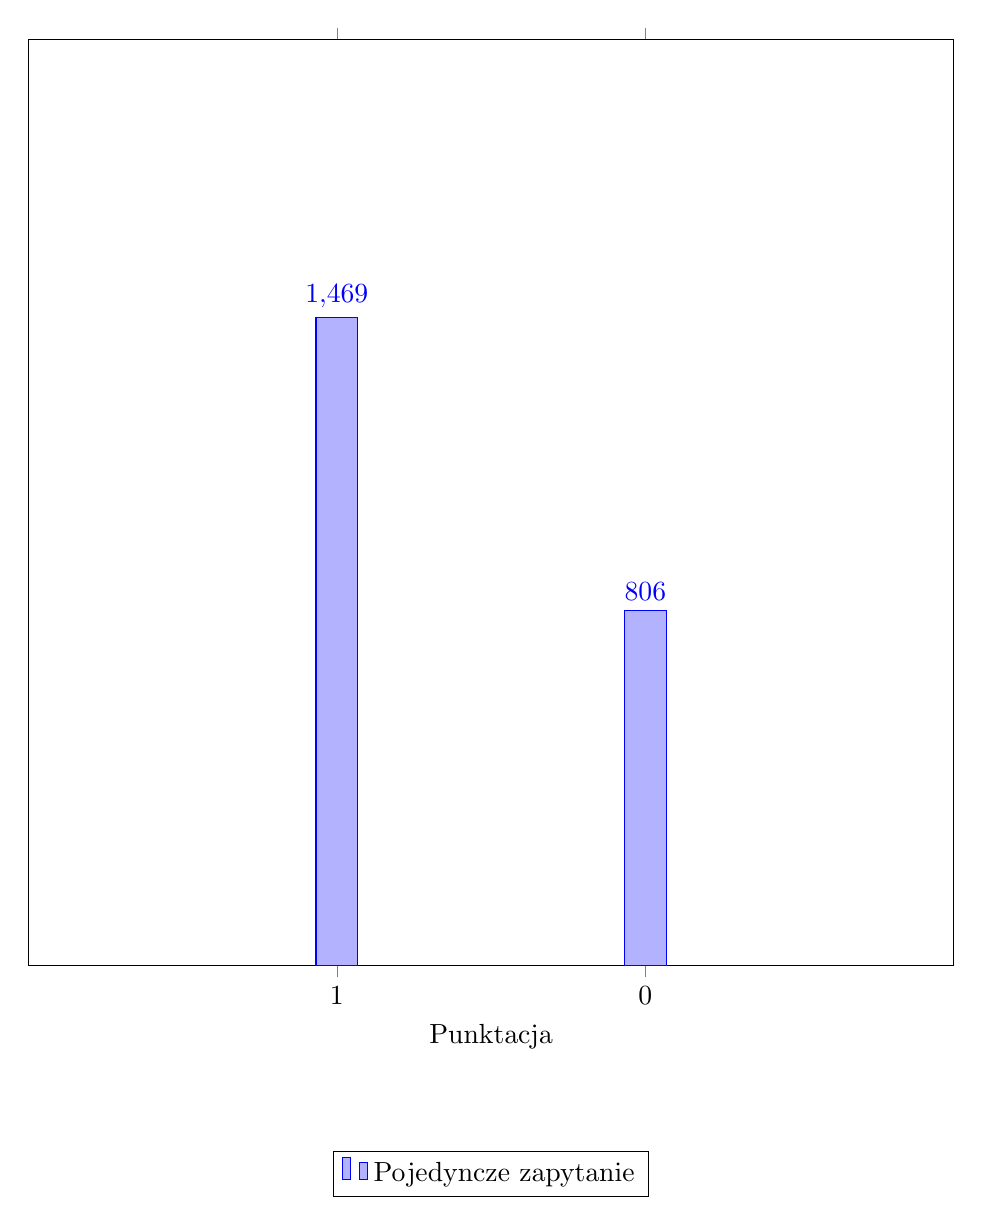
\begin{tikzpicture}
\begin{axis}[
    ybar,
    symbolic x coords={1, 0},
    xtick=data,
    %ylabel={Liczba},
    width=1.1\textwidth,
    height=1.1\textwidth,
    ytick = \empty,
    nodes near coords,
    bar width=15pt,
    enlarge x limits=1,
    ymin=0,
    ymax=2100,
    xlabel={Punktacja},
    legend style={at={(0.5,-0.20)}, anchor=north, legend columns=-1}
]
\addplot coordinates {(1,1469) (0,806)};
\addlegendentry{Pojedyncze zapytanie}
\end{axis}
\end{tikzpicture}
\end{minipage}
\caption{Wykres ocenionych wyników dla kategorii \textbf{Funkcja celu}.}
\end{figure}

W powyższym przykładzie widać całkowitą przewagę w ocenie obu wyników, która wskazuje na przewagę modelu  \textit{ZIMPL} stworzonego przez dostosowany do tego generator. Znacznie większą różnicę prezentują wygenerowane ograniczenia, co zostało przedstawione w wizualizacji poniżej. Pojedyncze zapytanie w każdym z przypadków testowych generuje kod zwierający w sobie niepoprawną deklarację ograniczenia, przez co nigdy nie został sklasyfikowany jako poprawny.

\begin{table}[ht]
\caption{Tabela ocenionych wyników dla kategorii \textbf{Ograniczenia}.}\label{tab:tabela14}
\centering%
\begin{tabular}{|l|c|c|}
\hline
\textbf{Punktacja} & \textbf{Generator} & \textbf{Pojedyncze zapytanie}\\
\hline
1 & 2140 & 1754 \\
\hline
0 & 0 & 2275 \\
\hline
Średnia ocena & 0,94 & 0,00 \\
\hline
\end{tabular}
\end{table}

\begin{figure}[H]
\centering
\begin{minipage}{0.45\textwidth}
\centering
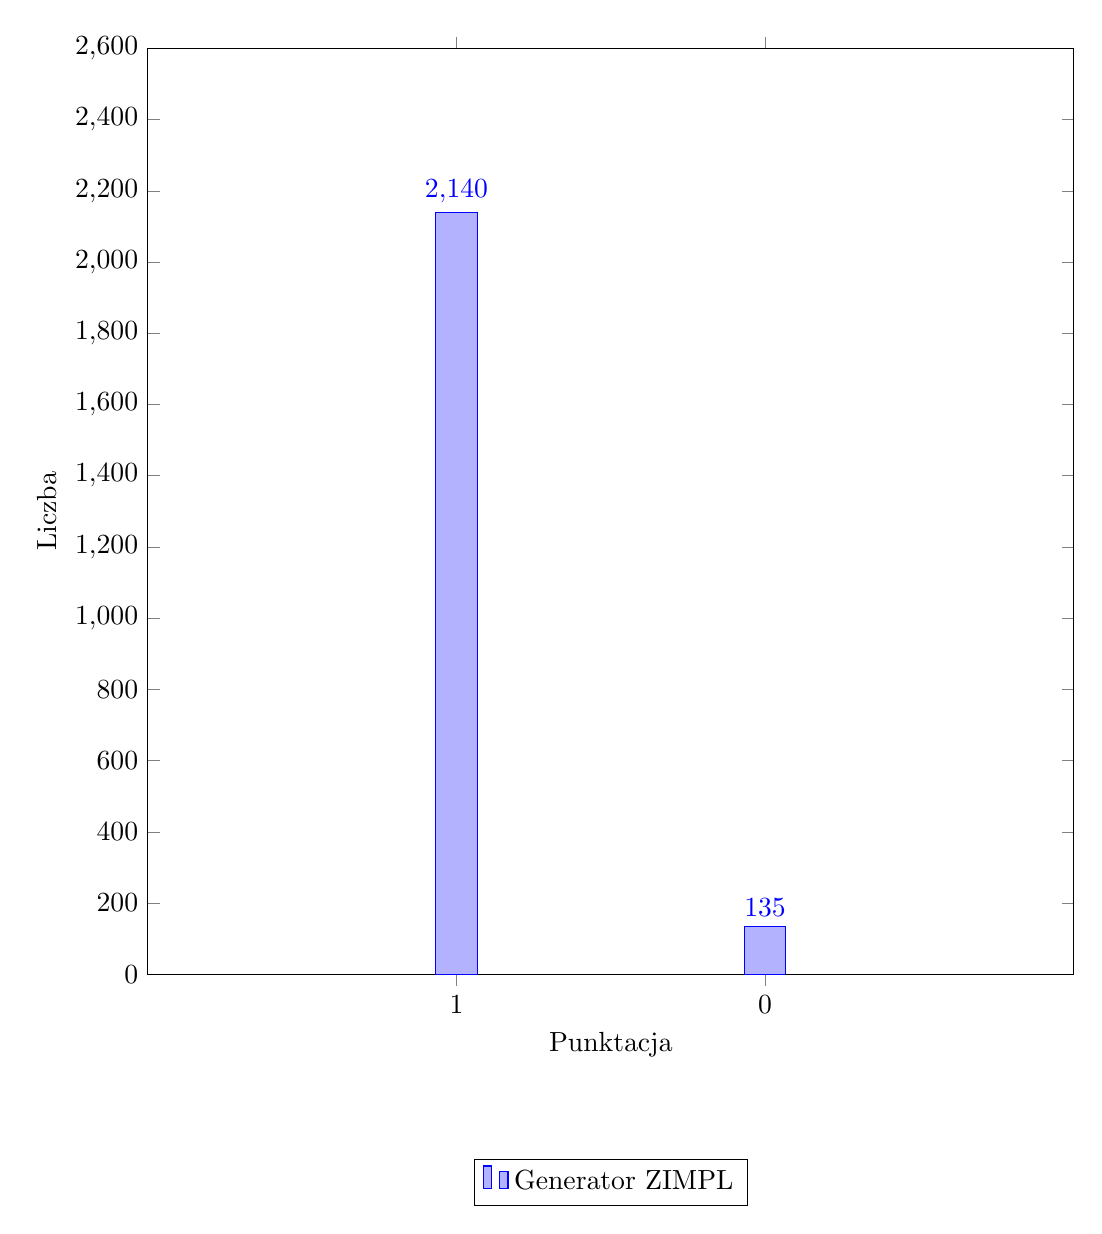
\begin{tikzpicture}
\begin{axis}[
    ybar,
    symbolic x coords={1, 0},
    xtick=data,
    ylabel={Liczba},
    width=1.1\textwidth,
    height=1.1\textwidth,
    nodes near coords,
    bar width=15pt,
    enlarge x limits=1,
    ymin=0,
    ymax=2600,
    xlabel={Punktacja},
    legend style={at={(0.5,-0.20)}, anchor=north, legend columns=-1}
]
\addplot coordinates {(1,2140) (0,135)};
\addlegendentry{Generator ZIMPL}
\end{axis}
\end{tikzpicture}
\end{minipage}%
\hspace{0.05\textwidth}
\begin{minipage}{0.45\textwidth}
\centering
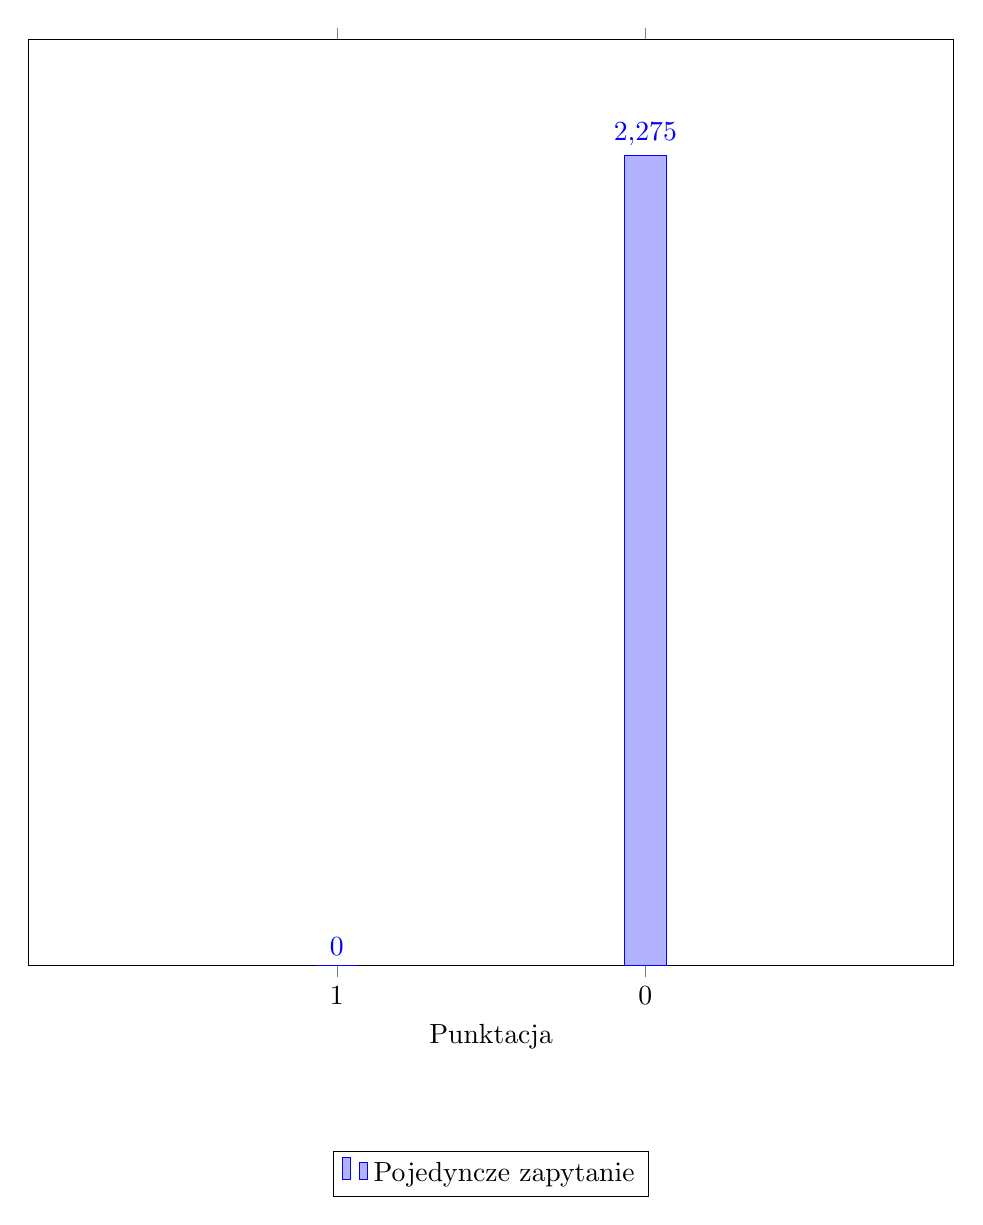
\begin{tikzpicture}
\begin{axis}[
    ybar,
    symbolic x coords={1, 0},
    xtick=data,
    %ylabel={Liczba},
    width=1.1\textwidth,
    height=1.1\textwidth,
    ytick = \empty,
    nodes near coords,
    bar width=15pt,
    enlarge x limits=1,
    ymin=0,
    ymax=2600,
    xlabel={Punktacja},
    legend style={at={(0.5,-0.20)}, anchor=north, legend columns=-1}
]
\addplot coordinates {(1,0) (0,2275)};
\addlegendentry{Pojedyncze zapytanie}
\end{axis}
\end{tikzpicture}
\end{minipage}
\caption{Wykres ocenionych wyników dla kategorii \textbf{Ograniczenia}.}
\end{figure}

Największą trudnością dla obu modeli jest uzyskanie pozytywnej punktacji w kategorii \textbf{Inne wymagania}. Wpływa na to fakt, iż jest to kategoria sprawdzająca wszystkie, wcześniej nieuwzględnione błędy, a zatem łatwo w niej stracić punkt. Również w tym przypadku generator okazał się nieco lepszy.

\begin{table}[ht]
\caption{Tabela ocenionych wyników dla kategorii \textbf{Inne wymagania}.}\label{tab:tabela15}
\centering%
\begin{tabular}{|l|c|c|}
\hline
\textbf{Punktacja} & \textbf{Generator} & \textbf{Pojedyncze zapytanie}\\
\hline
1 & 1665 & 1229 \\
\hline
0 & 610 & 1046 \\
\hline
Średnia ocena & 0,73 & 0,54 \\
\hline
\end{tabular}
\end{table}


\begin{figure}[H]
\centering
\begin{minipage}{0.45\textwidth}
\centering
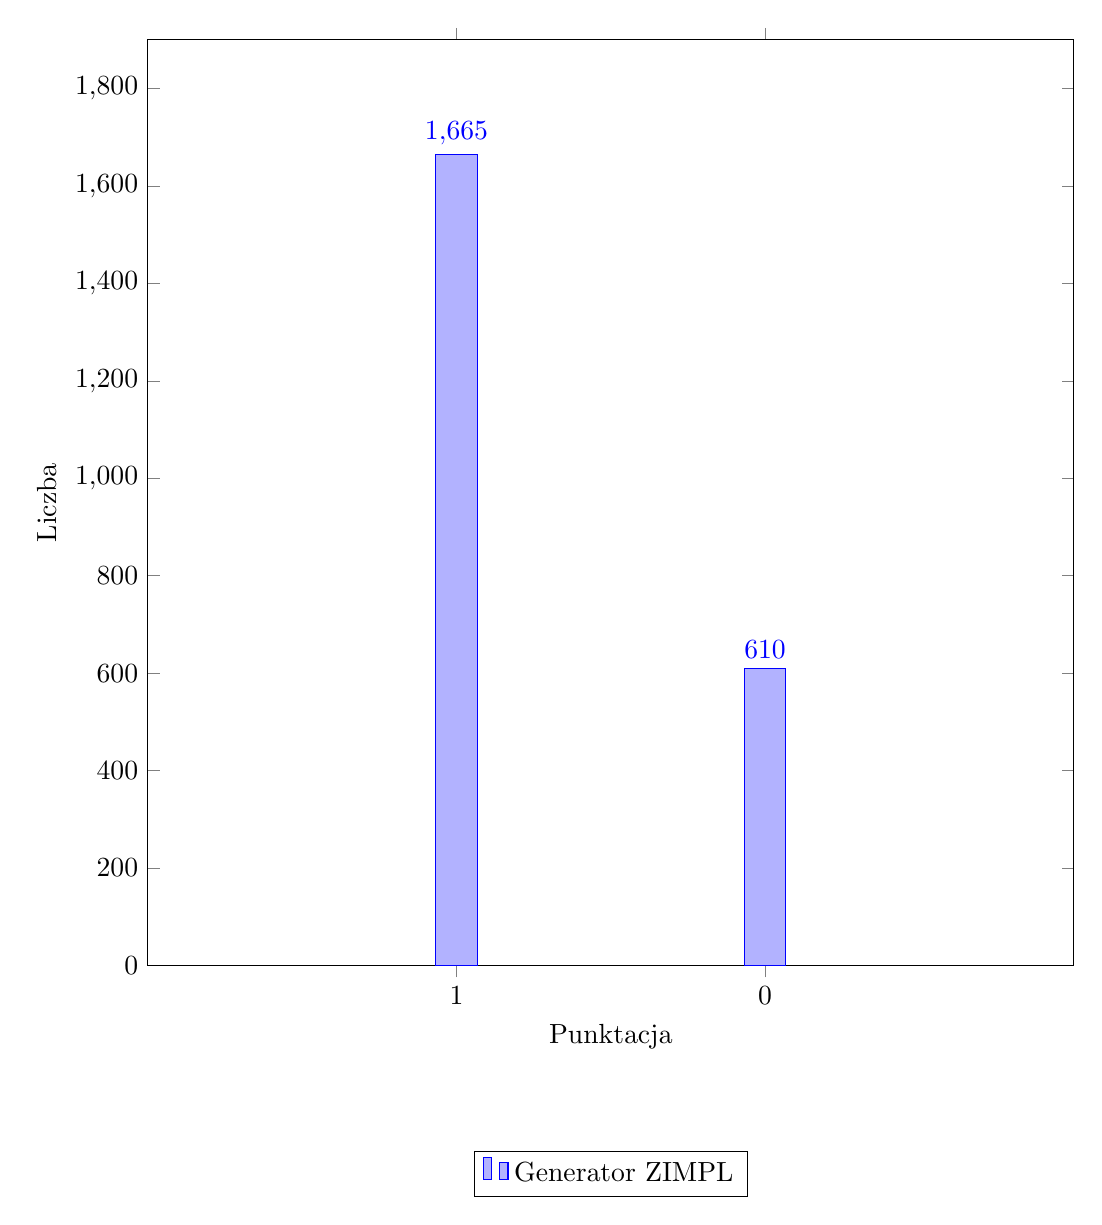
\begin{tikzpicture}
\begin{axis}[
    ybar,
    symbolic x coords={1, 0},
    xtick=data,
    ylabel={Liczba},
    width=1.1\textwidth,
    height=1.1\textwidth,
    nodes near coords,
    bar width=15pt,
    enlarge x limits=1,
    ymin=0,
    ymax=1900,
    xlabel={Punktacja},
    legend style={at={(0.5,-0.20)}, anchor=north, legend columns=-1}
]
\addplot coordinates {(1,1665) (0,610)};
\addlegendentry{Generator ZIMPL}
\end{axis}
\end{tikzpicture}
\end{minipage}%
\hspace{0.05\textwidth}
\begin{minipage}{0.45\textwidth}
\centering
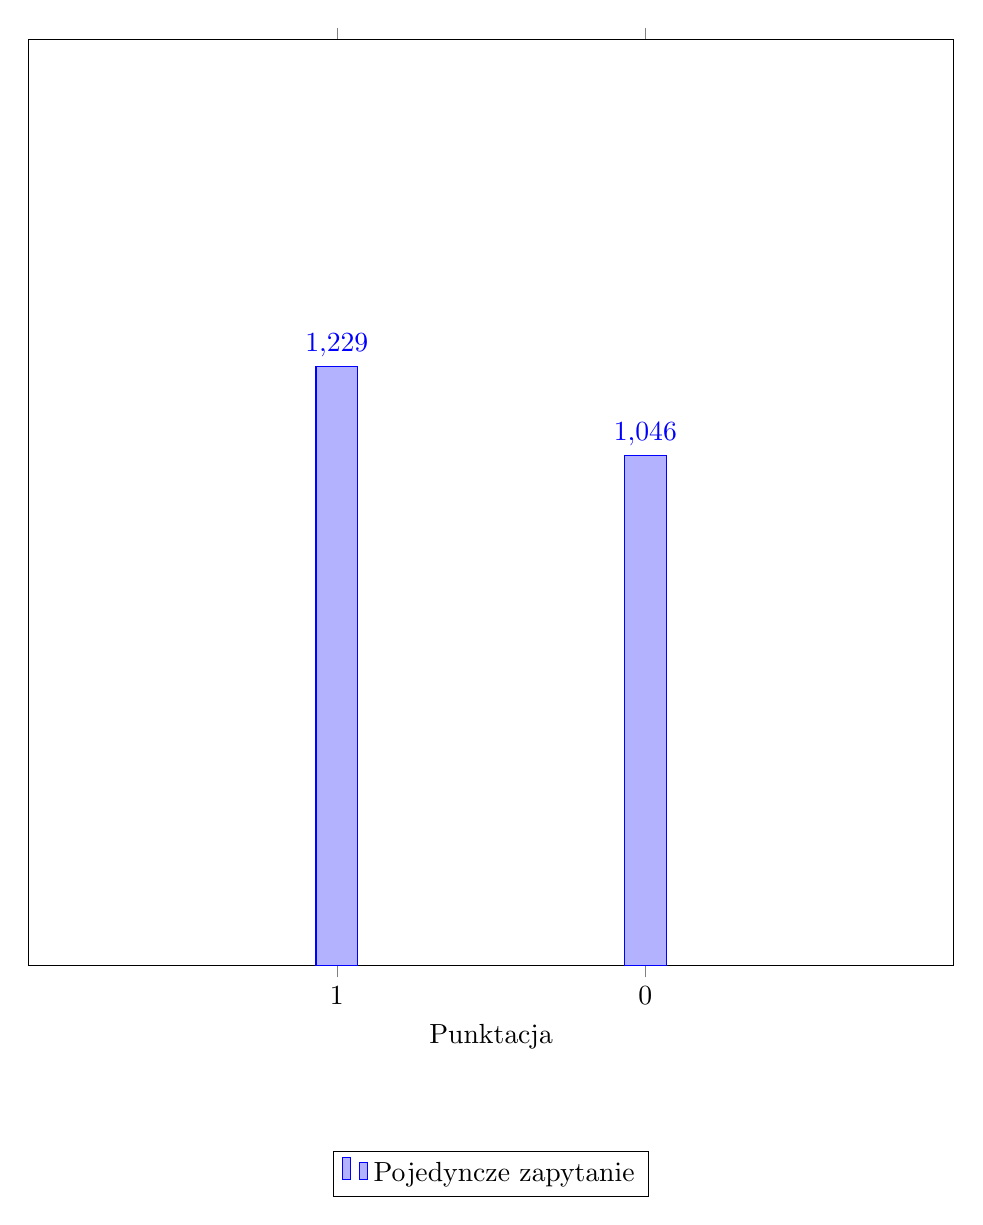
\begin{tikzpicture}
\begin{axis}[
    ybar,
    symbolic x coords={1, 0},
    xtick=data,
    %ylabel={Liczba},
    width=1.1\textwidth,
    height=1.1\textwidth,
    ytick = \empty,
    nodes near coords,
    bar width=15pt,
    enlarge x limits=1,
    ymin=0,
    ymax=1900,
    xlabel={Punktacja},
    legend style={at={(0.5,-0.20)}, anchor=north, legend columns=-1}
]
\addplot coordinates {(1,1229) (0,1046)};
\addlegendentry{Pojedyncze zapytanie}
\end{axis}
\end{tikzpicture}
\end{minipage}
\caption{Wykres ocenionych wyników dla kategorii \textbf{Inne wymagania}.}
\end{figure}

Wyniki zapewnianie dla sztywnego formułowania modeli  \textit{ZIMPL} zapewniają poprawę, ale nie jest ona tak wysoka, jak przy parametryzowanych danych. W średnio wyniki otrzymują ocenę w 3,31, podczas gdy dla pojedynczego zapytania ten wynik zmniejsza się o 1,50 punktu (średnio 1,81).

\begin{table}[ht]
\caption{Tabela sumarycznej oceny wyników dla kodowanych sztywno modeli.}\label{tab:tabela16}
\centering%
\begin{tabular}{|l|c|c|}
\hline
\textbf{Punktacja} & \textbf{Generator} & \textbf{Pojedyncze zapytanie}\\
\hline
0 & 103 & 509 \\
\hline
1 & 46 & 442 \\
\hline
2 & 386 & 298 \\
\hline
3 & 259 & 1026 \\
\hline
4 & 1481 & 0 \\
\hline
\textbf{Średnia ocena} & \textbf{3,31} & \textbf{1,81} \\
\hline
\end{tabular}
\end{table}

\begin{figure}[H]
\centering
\begin{minipage}{0.45\textwidth}
\centering
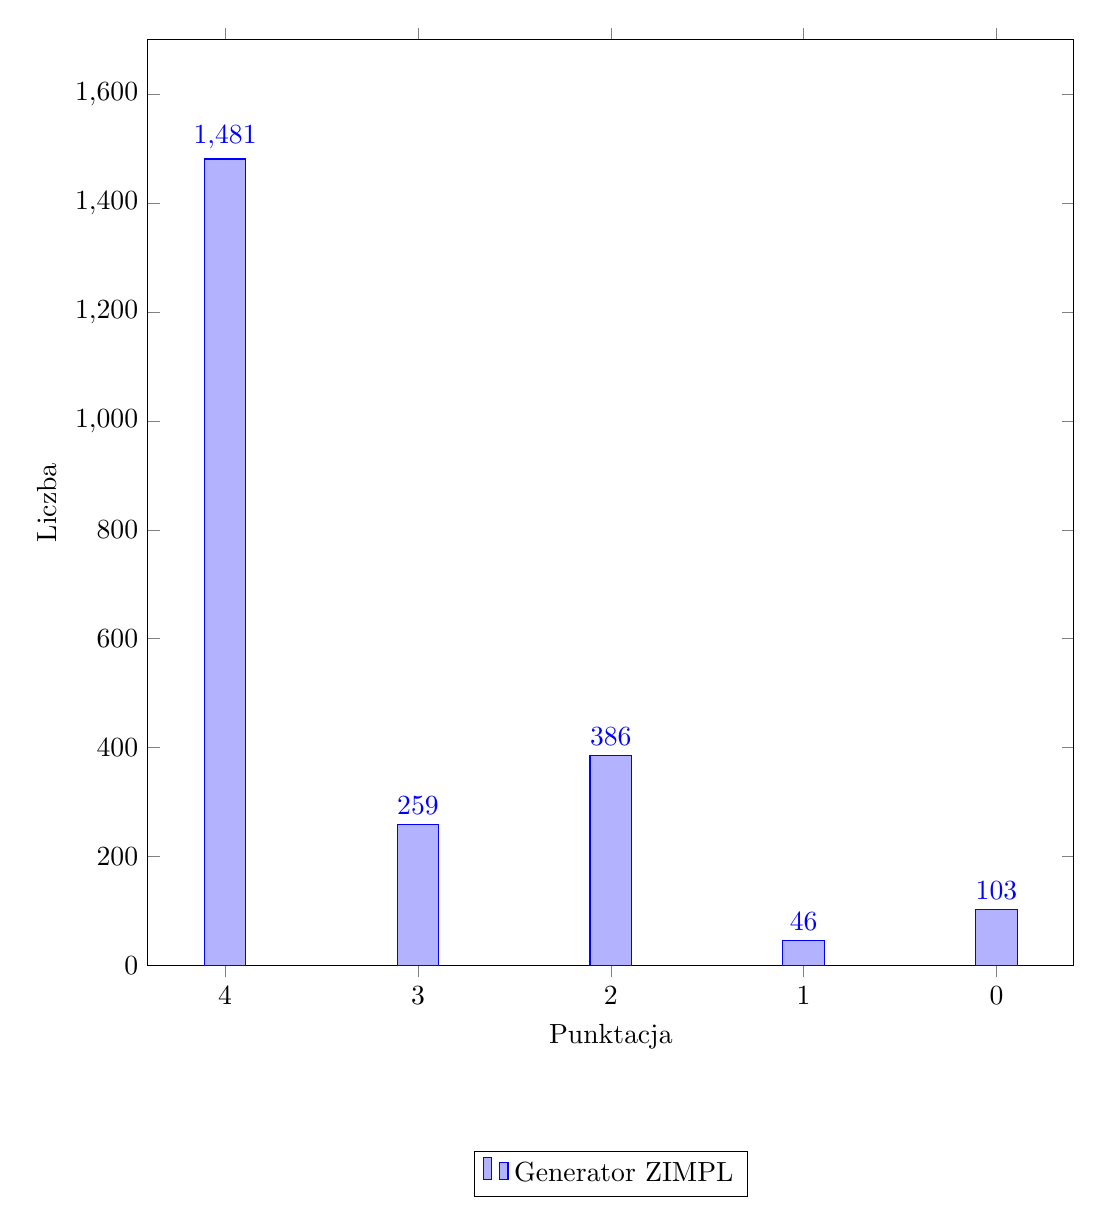
\begin{tikzpicture}
\begin{axis}[
    ybar,
    symbolic x coords={4,3,2,1,0},
    xtick=data,
    ylabel={Liczba},
    width=1.1\textwidth,
    height=1.1\textwidth,
    nodes near coords,
    bar width=15pt,
    ymin=0,
    ymax=1700,
    xlabel={Punktacja},
    legend style={at={(0.5,-0.20)}, anchor=north, legend columns=-1}
]
\addplot coordinates {(4,1481) (3,259) (2,386) (1,46) (0,103)};
\addlegendentry{Generator ZIMPL}
\end{axis}
\end{tikzpicture}
\end{minipage}%
\hspace{0.05\textwidth}
\begin{minipage}{0.45\textwidth}
\centering
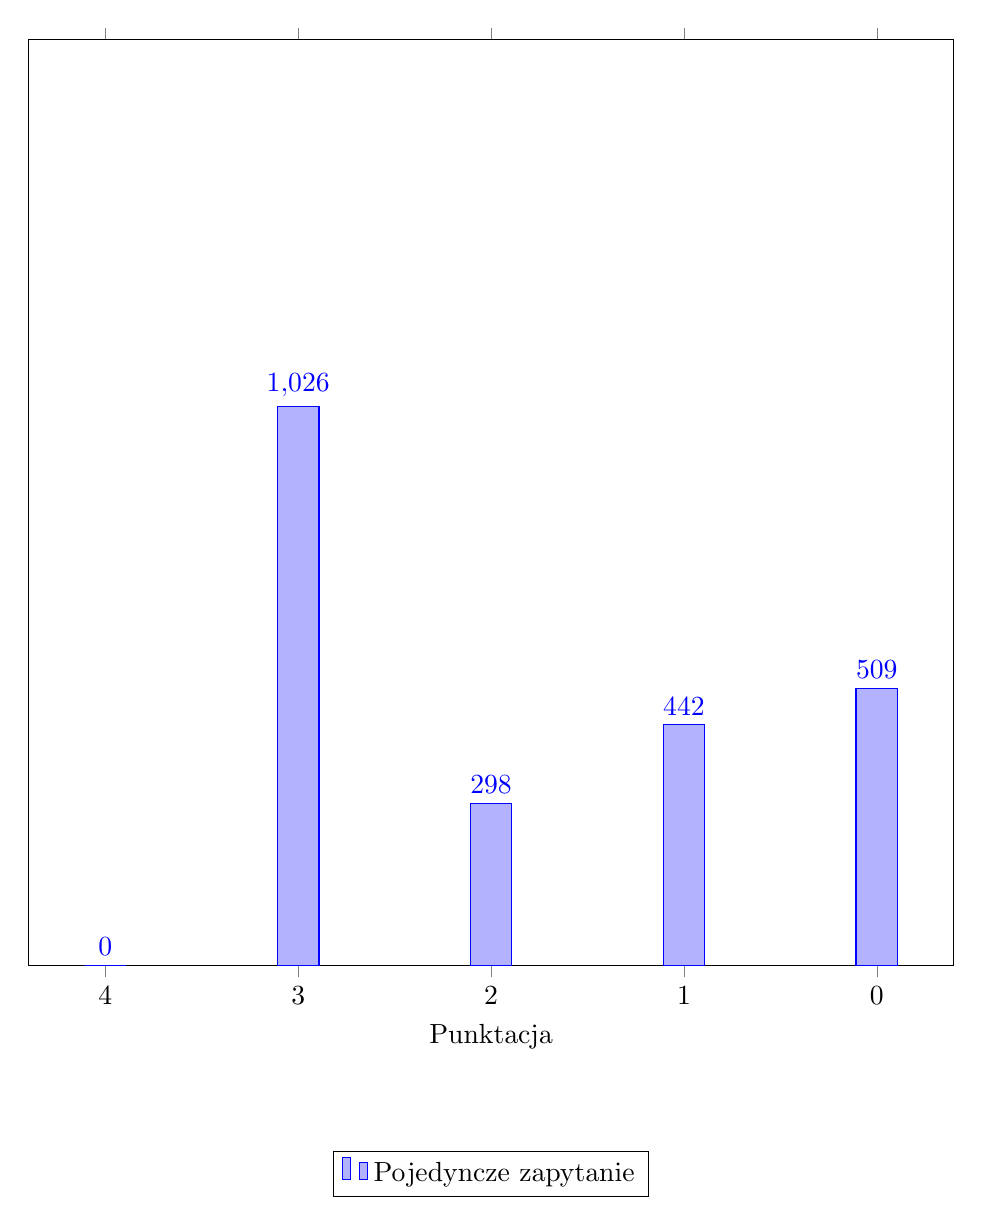
\begin{tikzpicture}
\begin{axis}[
    ybar,
    symbolic x coords={4,3,2,1,0},
    xtick=data,
    %ylabel={Liczba},
    width=1.1\textwidth,
    height=1.1\textwidth,
    ytick = \empty,
    nodes near coords,
    bar width=15pt,
    ymin=0,
    ymax=1700,
    xlabel={Punktacja},
    legend style={at={(0.5,-0.20)}, anchor=north, legend columns=-1}
]
\addplot coordinates {(4,0) (3,1026) (2,298) (1,442) (0,509)};
\addlegendentry{Pojedyncze zapytanie}
\end{axis}
\end{tikzpicture}
\end{minipage}
\caption{Wykres prezentujący sumaryczną ocenę wyników dla parametryzowanych modeli.}
\end{figure}

\subsection{Wyniki dla parametryzowanych modeli.}

Podobna analiza została przeprowadzona dla modeli parametryzowanych. Dla kategorii, jakie przedstawiają, przewaga generatora jest znacznie wyższa. Wynika to z złożoności kodu, z jakim pracuje. Modele generowane za pomocą pojedynczego zapytania nie posiadają wiedzy na temat struktury kodu, przez co mają problemy z identyfikacją zbiorów i parametrów. Punktacja w tym przypadku jest w kategoriach:

\begin{enumerate}
\item (1 punkt) \textbf{Definiowanie zbiorów} -- aby uzyskać punkt w tej kategorii, zbiory muszą być poprawnie zdefiniowane przy użyciu nawiasów klamrowych \texttt{{}}, z elementami w cudzysłowach. Każde odstępstwo od składni, powoduje utratę punktu.
\item (1 punkt) \textbf{Definiowanie parametrów} -- punkt jest przyznawany gdy parametry są poprawnie zindeksowane za pomocą nawiasów kwadratowych \texttt{[ ]} i logicznie zgodne z poprawnym kodem. Nazwy parametrów mogą się różnić, o ile zachowano ich poprawne zastosowanie i strukturę.
\item (1 punkt) \textbf{Definiowanie zmiennych} -- aby uzyskać punkt w tej kategorii, zmienne i typy muszą być zgodne ze sobą. Zmienne muszą być zgodne z odpowiednimi zbiorami. Ich nazwy i komentarze mogą się od siebie różnić, ale logika musi pozostać taka sama. Brak zgodności powoduje utratę punktu.
\item (1 punkt) \textbf{Funkcja celu} -- punkt przyznawany jest za poprawne zdefiniowanie funkcji celu. Musi być zgodna w strukturze, współczynnikach oraz poprawnie zdefiniowana za pomocą uwzględnienia minimalizacji lub maksymalizacji. Brak nazwy lub niezgodna struktura powodują utratę punktu.
\item (1 punkt) \textbf{Ograniczenia} -- aby otrzymać punkt, ograniczenia muszą być zdefiniowane zgodnie z poprawnym kodem. Liczba, logika i zapis muszą być zgodne, a każde ograniczenie powinno zaczynać się od \texttt{subto <nazwa>:}. Zastosowanie innej struktury powoduje odjęcie punktu.
\item (1 punkt) \textbf{Inne wymagania} -- punkt przyznaje się za spełnienie wymagań takich jak: użycie \texttt{\#} jako prefiksu komentarzy, brak zbędnych poleceń oraz poprawne rozpoczęcie każdej linii od jednego z kluczowych słów (\texttt{var}, \texttt{minimize}, \texttt{maximize}, \texttt{subto}).
\end{enumerate}

Już w pierwszej kategorii widać znaczącą różnicę w wynikach między generowanymi wynikami. Pojedyncze zapytanie nie radzi sobie z tworzeniem zbiorów, stosując błędną implementację. Średnie wyniki uzyskanej punktacji różnią się od siebie o \textbf{0,33} punktu, co jest najwyższym dotąd uzyskanym wynikiem.

\begin{table}[ht]
\caption{Tabela ocenionych wyników dla kategorii \textbf{Definiowanie zbiorów}.}\label{tab:tabela17}
\centering%
\begin{tabular}{|l|c|c|}
\hline
\textbf{Punktacja} & \textbf{Generator} & \textbf{Pojedyncze zapytanie}\\
\hline
1 & 1783 & 914 \\
\hline
0 & 242 & 1111 \\
\hline
Średnia ocena & 0,88 & 0,45 \\
\hline
\end{tabular}
\end{table}


\begin{figure}[H]
\centering
\begin{minipage}{0.45\textwidth}
\centering
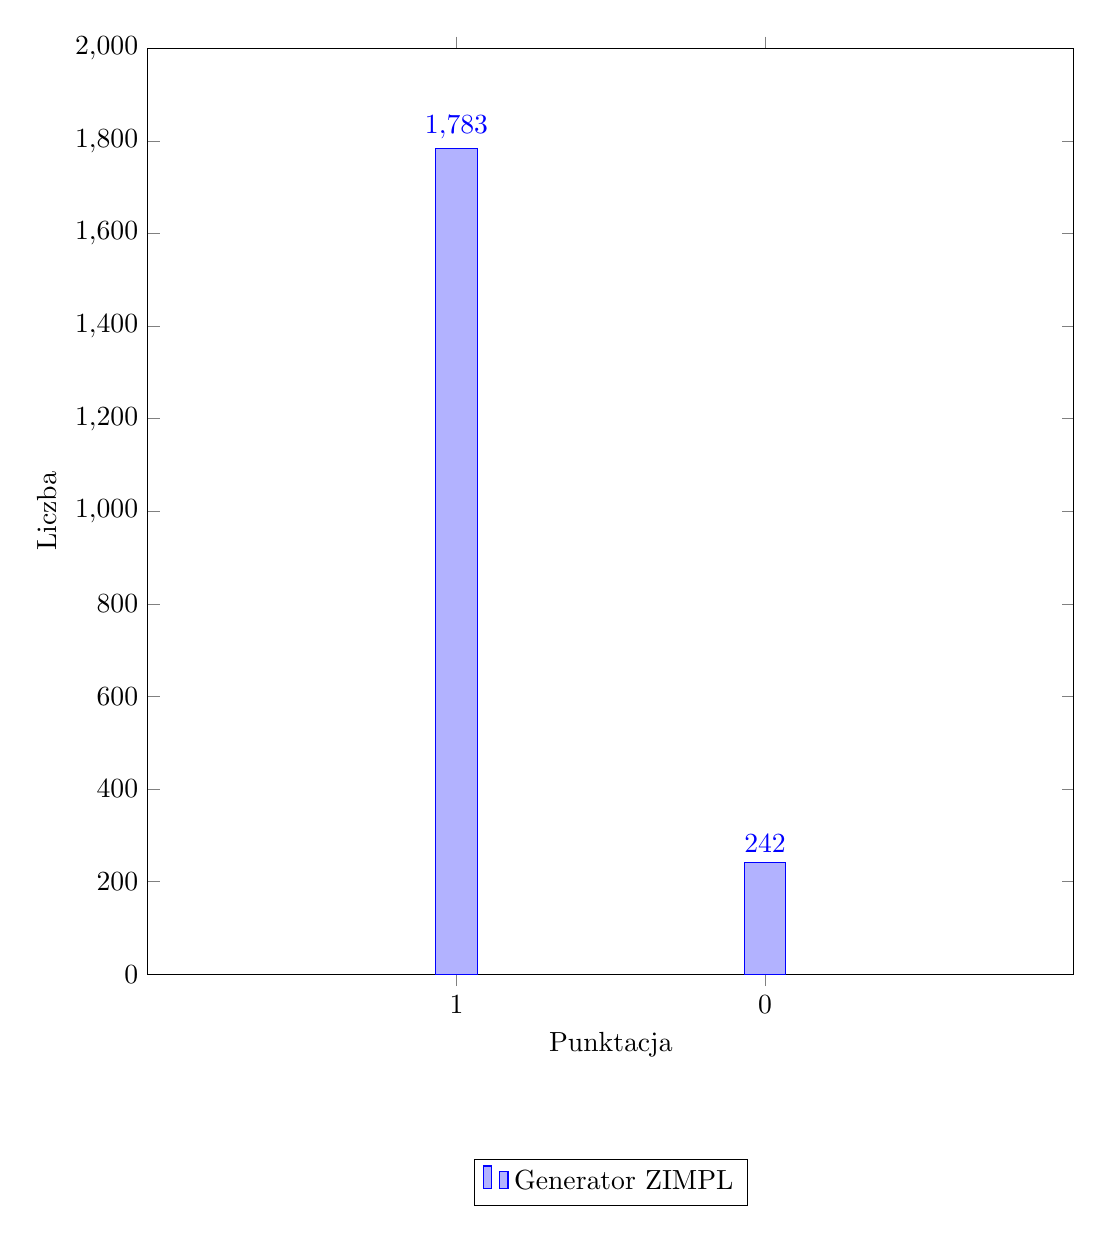
\begin{tikzpicture}
\begin{axis}[
    ybar,
    symbolic x coords={1, 0},
    xtick=data,
    ylabel={Liczba},
    width=1.1\textwidth,
    height=1.1\textwidth,
    nodes near coords,
    bar width=15pt,
    enlarge x limits=1,
    ymin=0,
    ymax=2000,
    xlabel={Punktacja},
    legend style={at={(0.5,-0.20)}, anchor=north, legend columns=-1}
]
\addplot coordinates {(1,1783) (0,242)};
\addlegendentry{Generator ZIMPL}
\end{axis}
\end{tikzpicture}
\end{minipage}%
\hspace{0.05\textwidth}
\begin{minipage}{0.45\textwidth}
\centering
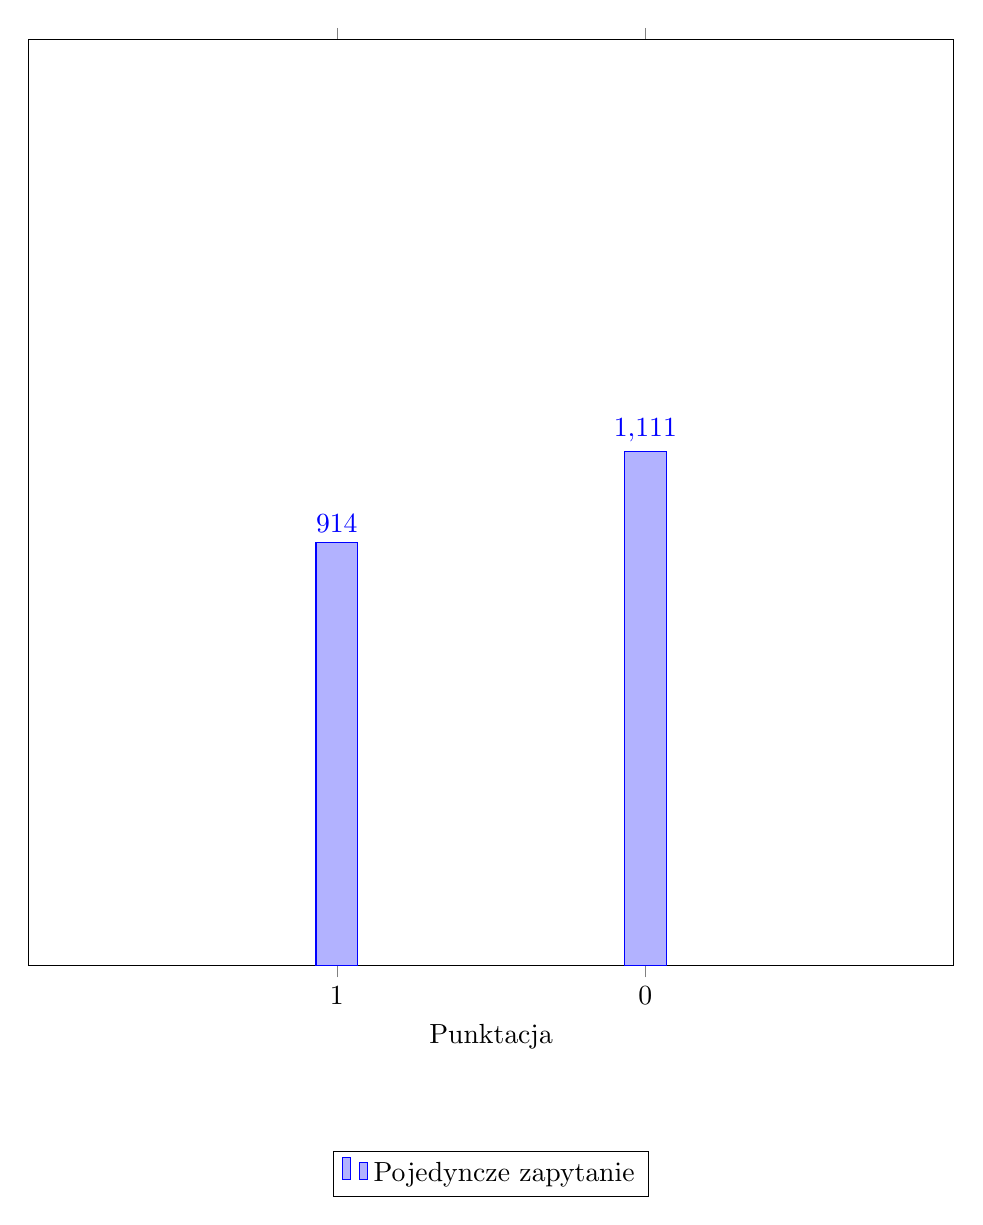
\begin{tikzpicture}
\begin{axis}[
    ybar,
    symbolic x coords={1, 0},
    xtick=data,
    %ylabel={Liczba},
    width=1.1\textwidth,
    height=1.1\textwidth,
    ytick = \empty,
    nodes near coords,
    bar width=15pt,
    enlarge x limits=1,
    ymin=0,
    ymax=2000,
    xlabel={Punktacja},
    legend style={at={(0.5,-0.20)}, anchor=north, legend columns=-1}
]
\addplot coordinates {(1,914) (0,1111)};
\addlegendentry{Pojedyncze zapytanie}
\end{axis}
\end{tikzpicture}
\end{minipage}
\caption{Wykres ocenionych wyników dla kategorii \textbf{Definiowanie zbiorów}.}
\end{figure}

Tworzenie parametrów prezentuje znacznie lepsze wyniki, zapewniając prawie 100\% skuteczności w tworzeniu przez generator. Wyniki pojedynczego zapytania również utrzymują się na poziomie powyżej 80\%.

\begin{table}[ht]
\caption{Tabela ocenionych wyników dla kategorii \textbf{Definiowanie parametrów}.}\label{tab:tabela18}
\centering%
\begin{tabular}{|l|c|c|}
\hline
\textbf{Punktacja} & \textbf{Generator} & \textbf{Pojedyncze zapytanie}\\
\hline
1 & 2008 & 1663 \\
\hline
0 & 17 & 362 \\
\hline
Średnia ocena & 0,99 & 0,82 \\
\hline
\end{tabular}
\end{table}

\begin{figure}[H]
\centering
\begin{minipage}{0.45\textwidth}
\centering
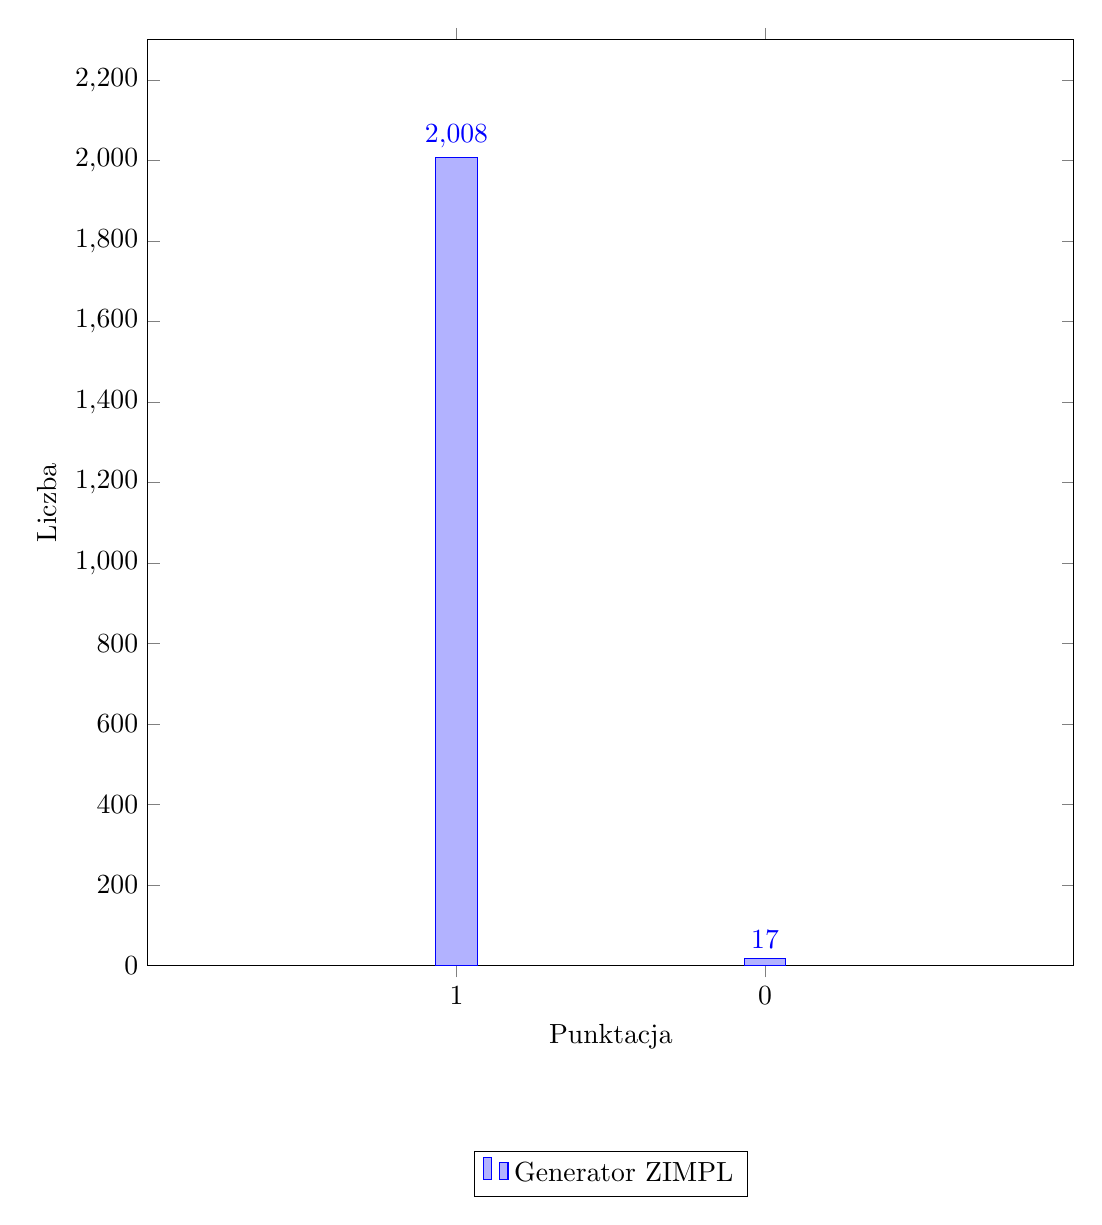
\begin{tikzpicture}
\begin{axis}[
    ybar,
    symbolic x coords={1, 0},
    xtick=data,
    ylabel={Liczba},
    width=1.1\textwidth,
    height=1.1\textwidth,
    nodes near coords,
    bar width=15pt,
    enlarge x limits=1,
    ymin=0,
    ymax=2300,
    xlabel={Punktacja},
    legend style={at={(0.5,-0.20)}, anchor=north, legend columns=-1}
]
\addplot coordinates {(1,2008) (0,17)};
\addlegendentry{Generator ZIMPL}
\end{axis}
\end{tikzpicture}
\end{minipage}%
\hspace{0.05\textwidth}
\begin{minipage}{0.45\textwidth}
\centering
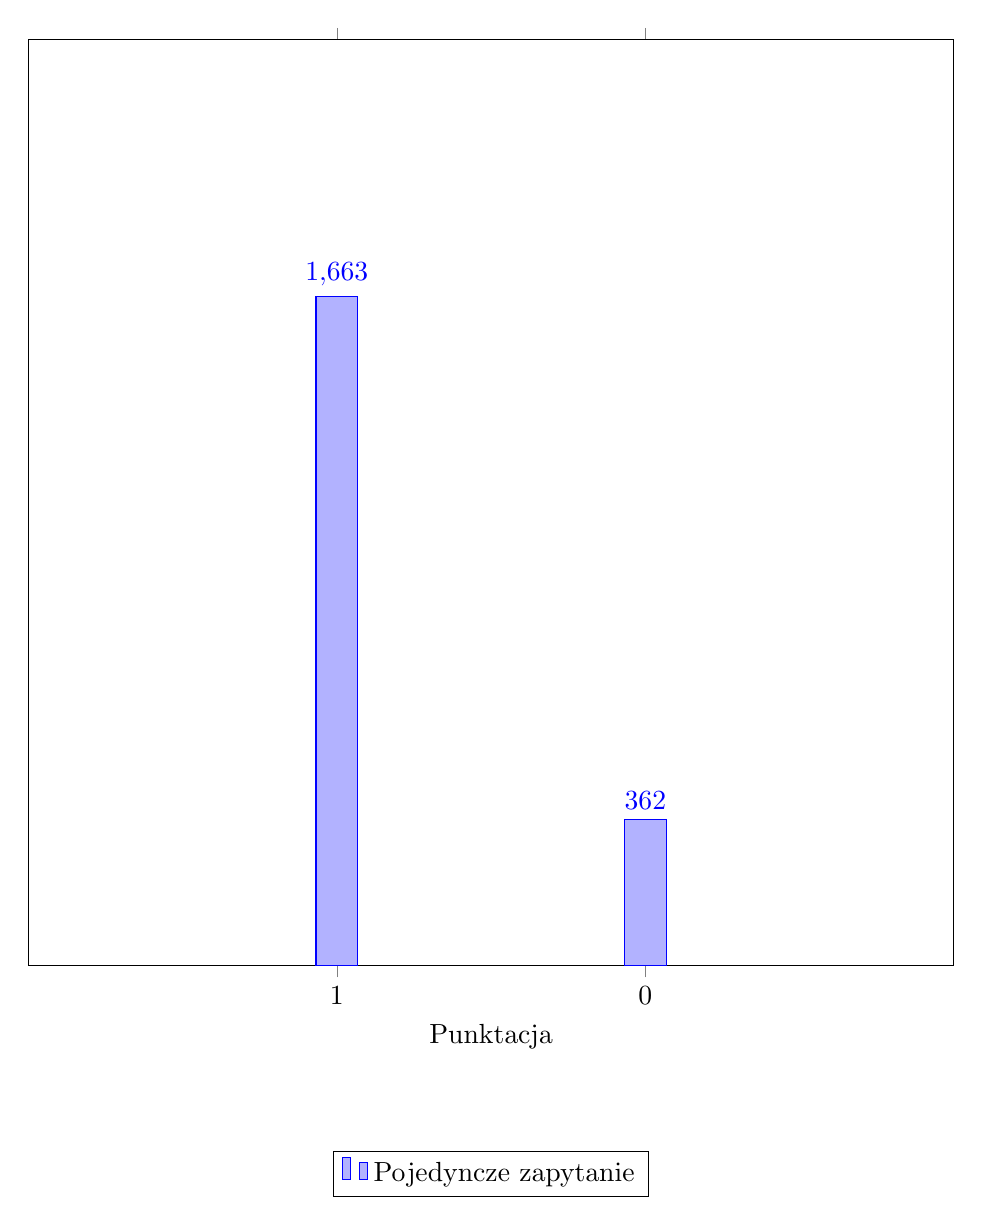
\begin{tikzpicture}
\begin{axis}[
    ybar,
    symbolic x coords={1, 0},
    xtick=data,
    %ylabel={Liczba},
    width=1.1\textwidth,
    height=1.1\textwidth,
    ytick = \empty,
    nodes near coords,
    bar width=15pt,
    enlarge x limits=1,
    ymin=0,
    ymax=2300,
    xlabel={Punktacja},
    legend style={at={(0.5,-0.20)}, anchor=north, legend columns=-1}
]
\addplot coordinates {(1,1663) (0,362)};
\addlegendentry{Pojedyncze zapytanie}
\end{axis}
\end{tikzpicture}
\end{minipage}
\caption{Wykres ocenionych wyników dla kategorii \textbf{Definiowanie parametrów}.}
\end{figure}

Definiowanie zmiennych na podstawie zbiorów i parametrów obniża jakość wyniku kodu, przez co nie zostaje osiągnięta 100\% poprawność, tak jak w przypadku sztywnego formatu kodu. Wyniki generatora w tym przypadku są nieznacznie wyższe.

\begin{table}[ht]
\caption{Tabela ocenionych wyników dla kategorii \textbf{Definiowanie zmiennnych}.}\label{tab:tabela19}
\centering%
\begin{tabular}{|l|c|c|}
\hline
\textbf{Punktacja} & \textbf{Generator} & \textbf{Pojedyncze zapytanie}\\
\hline
1 & 1713 & 1473 \\
\hline
0 & 312 & 552 \\
\hline
Średnia ocena & 0,85 & 0,73 \\
\hline
\end{tabular}
\end{table}

\begin{figure}[H]
\centering
\begin{minipage}{0.45\textwidth}
\centering
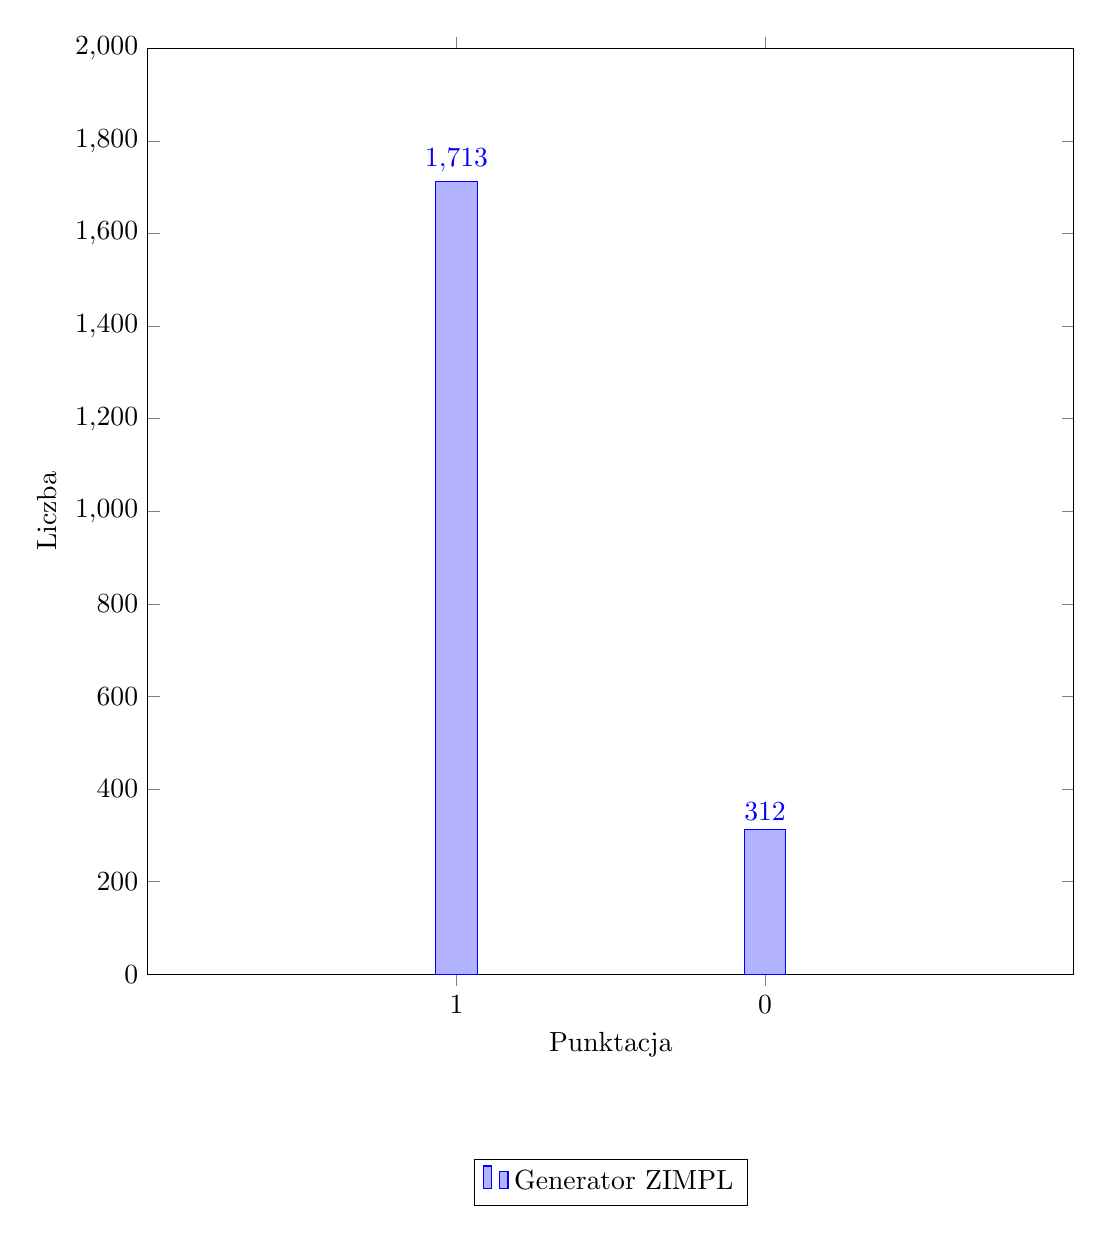
\begin{tikzpicture}
\begin{axis}[
    ybar,
    symbolic x coords={1, 0},
    xtick=data,
    ylabel={Liczba},
    width=1.1\textwidth,
    height=1.1\textwidth,
    nodes near coords,
    bar width=15pt,
    enlarge x limits=1,
    ymin=0,
    ymax=2000,
    xlabel={Punktacja},
    legend style={at={(0.5,-0.20)}, anchor=north, legend columns=-1}
]
\addplot coordinates {(1,1713) (0,312)};
\addlegendentry{Generator ZIMPL}
\end{axis}
\end{tikzpicture}
\end{minipage}%
\hspace{0.05\textwidth}
\begin{minipage}{0.45\textwidth}
\centering
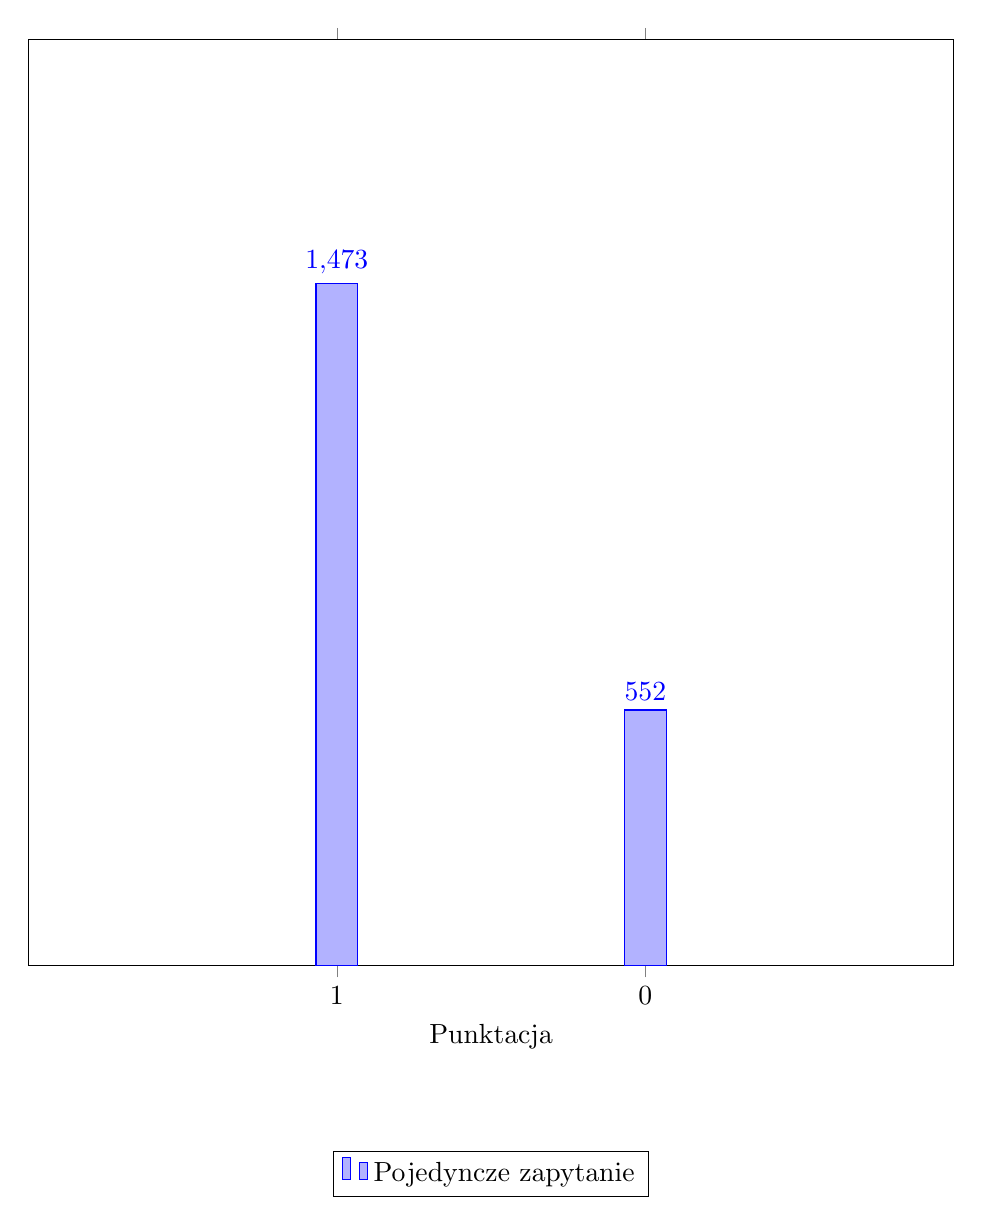
\begin{tikzpicture}
\begin{axis}[
    ybar,
    symbolic x coords={1, 0},
    xtick=data,
    xlabel={Punktacja},
    width=1.1\textwidth,
    height=1.1\textwidth,
    ytick = \empty,
    nodes near coords,
    bar width=15pt,
    enlarge x limits=1,
    ymin=0,
    ymax=2000,
    legend style={at={(0.5,-0.20)}, anchor=north, legend columns=-1}
]
\addplot coordinates {(1,1473) (0,552)};
\addlegendentry{Pojedyncze zapytanie}
\end{axis}
\end{tikzpicture}
\end{minipage}
\caption{Wykres ocenionych wyników dla kategorii \textbf{Definiowanie zmiennnych}.}
\end{figure}

Generowanie funkcji celu na podstawie wcześniej zdeklarowanych zmiennych działa bardzo dobrze, a wyniki posiadają poprawnie zdefiniowaną minimalizację/maksymalizację, a także prawidłowe sumowanie na zbiorach.

\begin{table}[ht]
\caption{Tabela ocenionych wyników dla kategorii \textbf{Funkcja celu}.}\label{tab:tabela20}
\centering%
\begin{tabular}{|l|c|c|}
\hline
\textbf{Punktacja} & \textbf{Generator} & \textbf{Pojedyncze zapytanie}\\
\hline
1 & 2002 & 2000 \\
\hline
0 & 23 & 25 \\
\hline
Średnia ocena & 0,83 & 0,65 \\
\hline
\end{tabular}
\end{table}

\begin{figure}[H]
\centering
\begin{minipage}{0.45\textwidth}
\centering
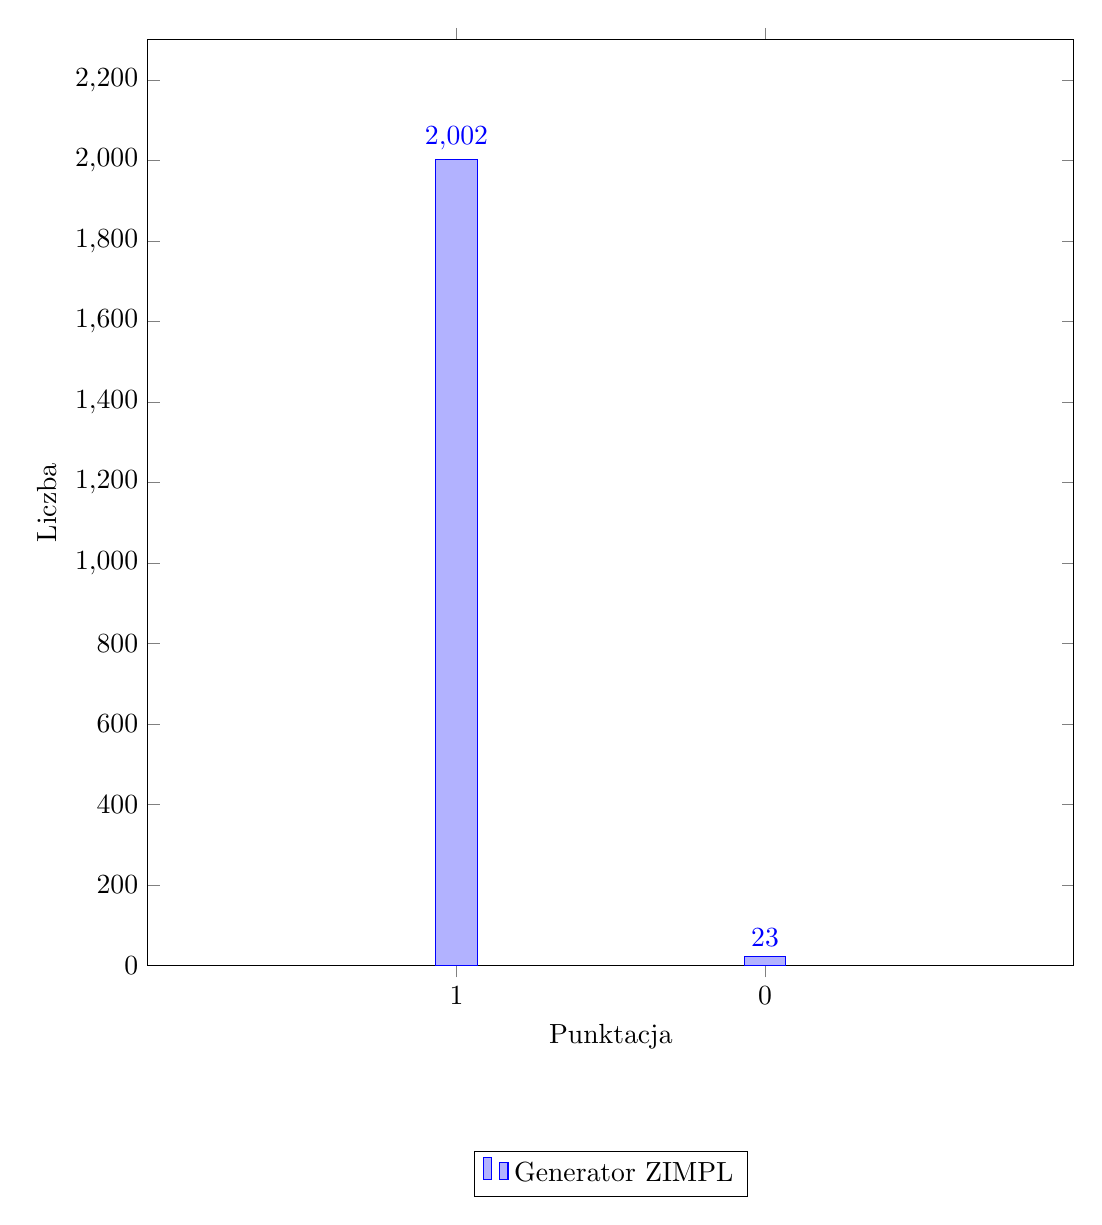
\begin{tikzpicture}
\begin{axis}[
    ybar,
    symbolic x coords={1, 0},
    xtick=data,
    ylabel={Liczba},
    width=1.1\textwidth,
    height=1.1\textwidth,
    nodes near coords,
    bar width=15pt,
    enlarge x limits=1,
    ymin=0,
    ymax=2300,
    xlabel={Punktacja},
    legend style={at={(0.5,-0.20)}, anchor=north, legend columns=-1}
]
\addplot coordinates {(1,2002) (0,23)};
\addlegendentry{Generator ZIMPL}
\end{axis}
\end{tikzpicture}
\end{minipage}%
\hspace{0.05\textwidth}
\begin{minipage}{0.45\textwidth}
\centering
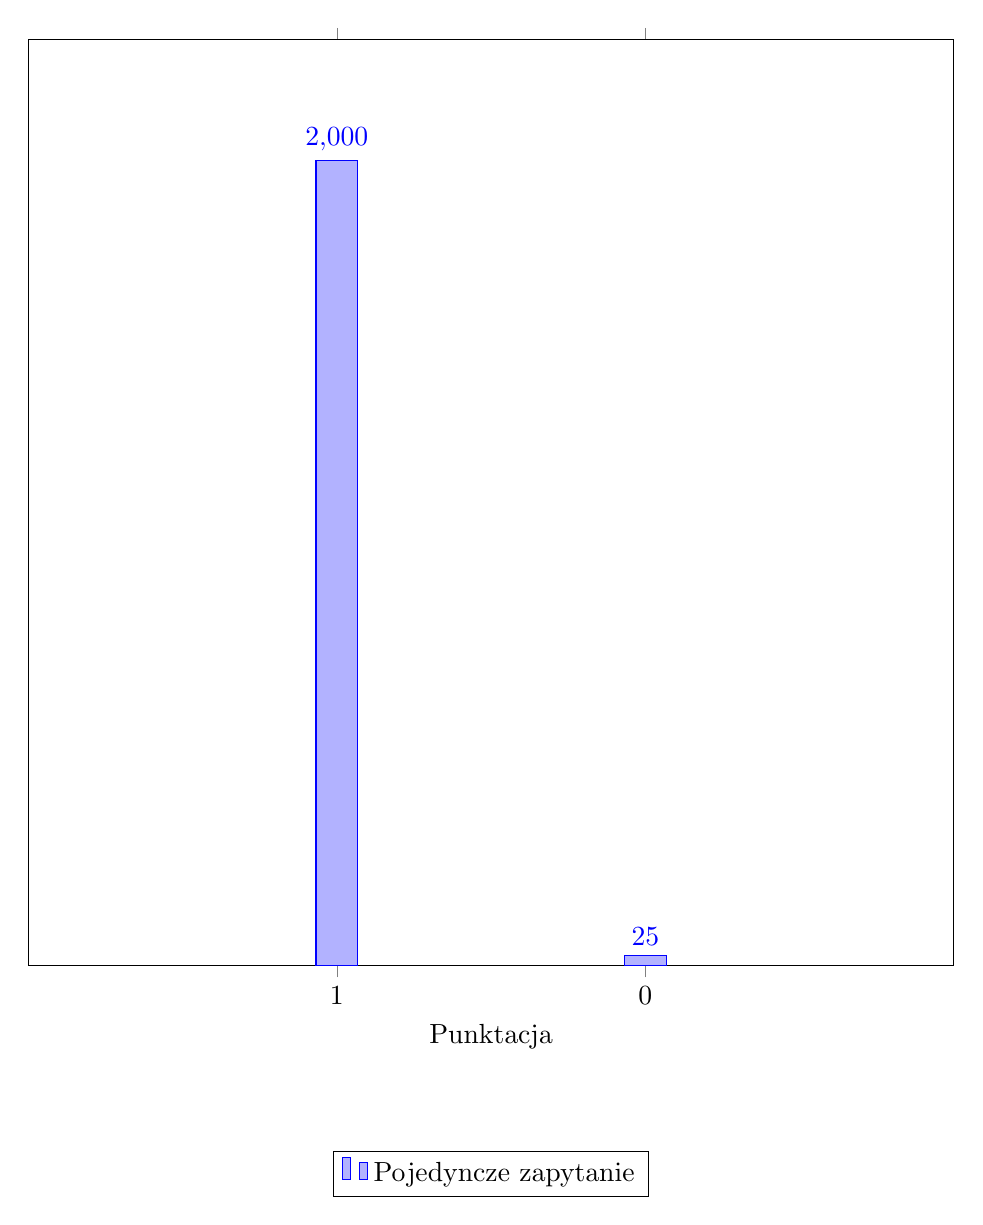
\begin{tikzpicture}
\begin{axis}[
    ybar,
    symbolic x coords={1, 0},
    xtick=data,
    %ylabel={Liczba},
    width=1.1\textwidth,
    height=1.1\textwidth,
    ytick = \empty,
    nodes near coords,
    bar width=15pt,
    enlarge x limits=1,
    ymin=0,
    ymax=2300,
    xlabel={Punktacja},
    legend style={at={(0.5,-0.20)}, anchor=north, legend columns=-1}
]
\addplot coordinates {(1,2000) (0,25)};
\addlegendentry{Pojedyncze zapytanie}
\end{axis}
\end{tikzpicture}
\end{minipage}
\caption{Wykres ocenionych wyników dla kategorii \textbf{Funkcja celu}.}
\end{figure}

Znacząca różnica pojawia się przy porównywaniu ograniczeń. Pojedyncze zapytanie nie zna składni kodu  \textit{ZIMPL}, w związku z czym każdorazowo deklaruje niepoprawne ograniczenia, używając takich elementów jak \texttt{s.t.} lub \texttt{subject to}.

\begin{table}[ht]
\caption{Tabela ocenionych wyników dla kategorii \textbf{Ograniczenia}.}\label{tab:tabela21}
\centering%
\begin{tabular}{|l|c|c|}
\hline
\textbf{Punktacja} & \textbf{Generator} & \textbf{Pojedyncze zapytanie}\\
\hline
1 & 1790 & 0 \\
\hline
0 & 235 & 2025 \\
\hline
Średnia ocena & 0,88 & 0,00 \\
\hline
\end{tabular}
\end{table}

\begin{figure}[H]
\centering
\begin{minipage}{0.45\textwidth}
\centering
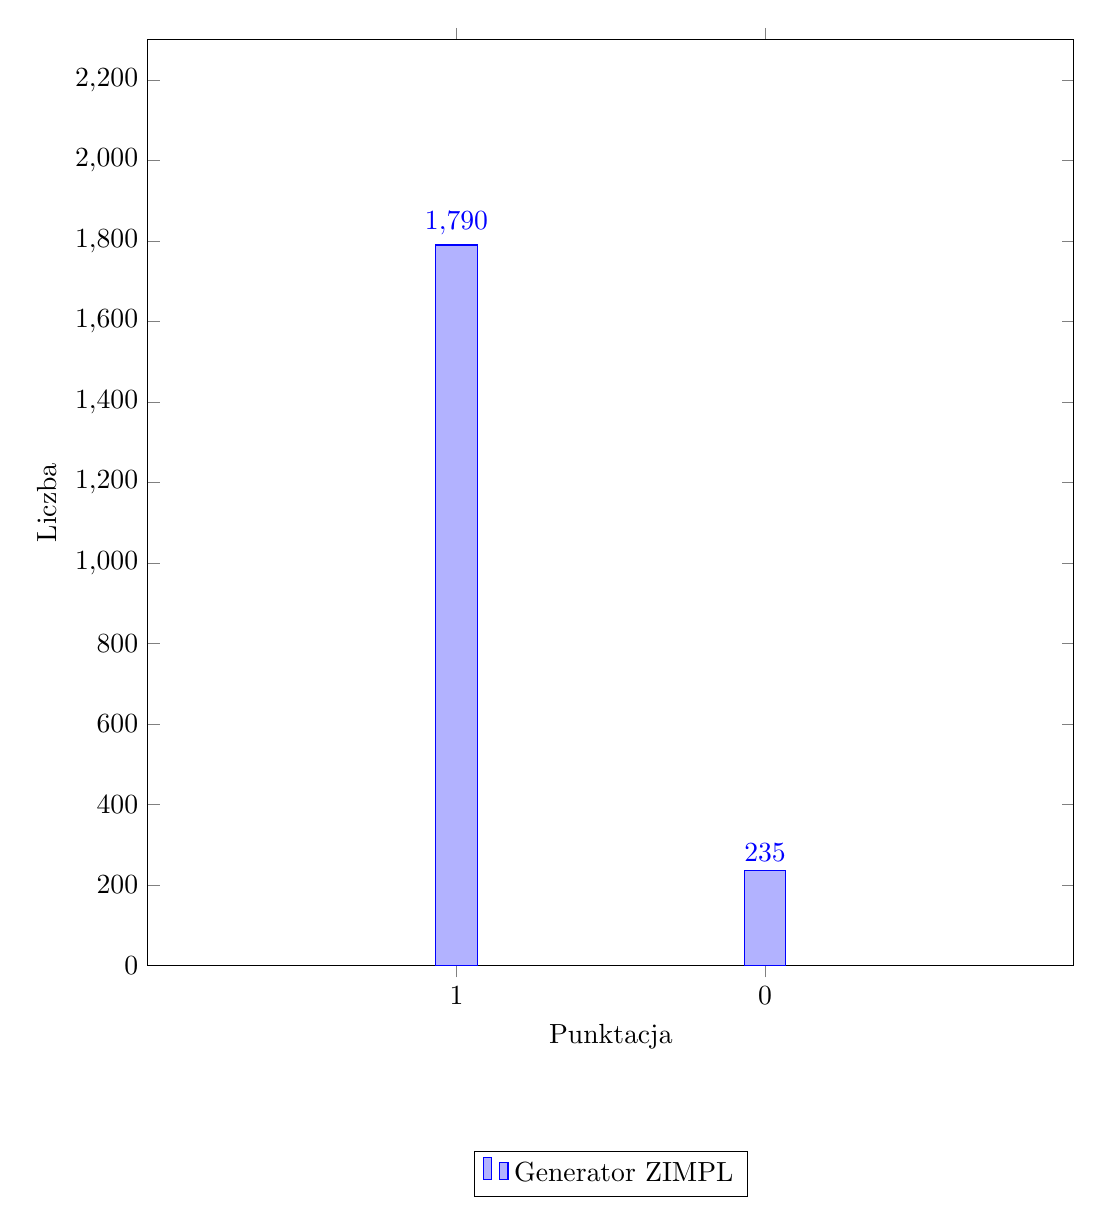
\begin{tikzpicture}
\begin{axis}[
    ybar,
    symbolic x coords={1, 0},
    xtick=data,
    ylabel={Liczba},
    width=1.1\textwidth,
    height=1.1\textwidth,
    nodes near coords,
    bar width=15pt,
    enlarge x limits=1,
    ymin=0,
    ymax=2300,
    xlabel={Punktacja},
    legend style={at={(0.5,-0.20)}, anchor=north, legend columns=-1}
]
\addplot coordinates {(1,1790) (0,235)};
\addlegendentry{Generator ZIMPL}
\end{axis}
\end{tikzpicture}
\end{minipage}%
\hspace{0.05\textwidth}
\begin{minipage}{0.45\textwidth}
\centering
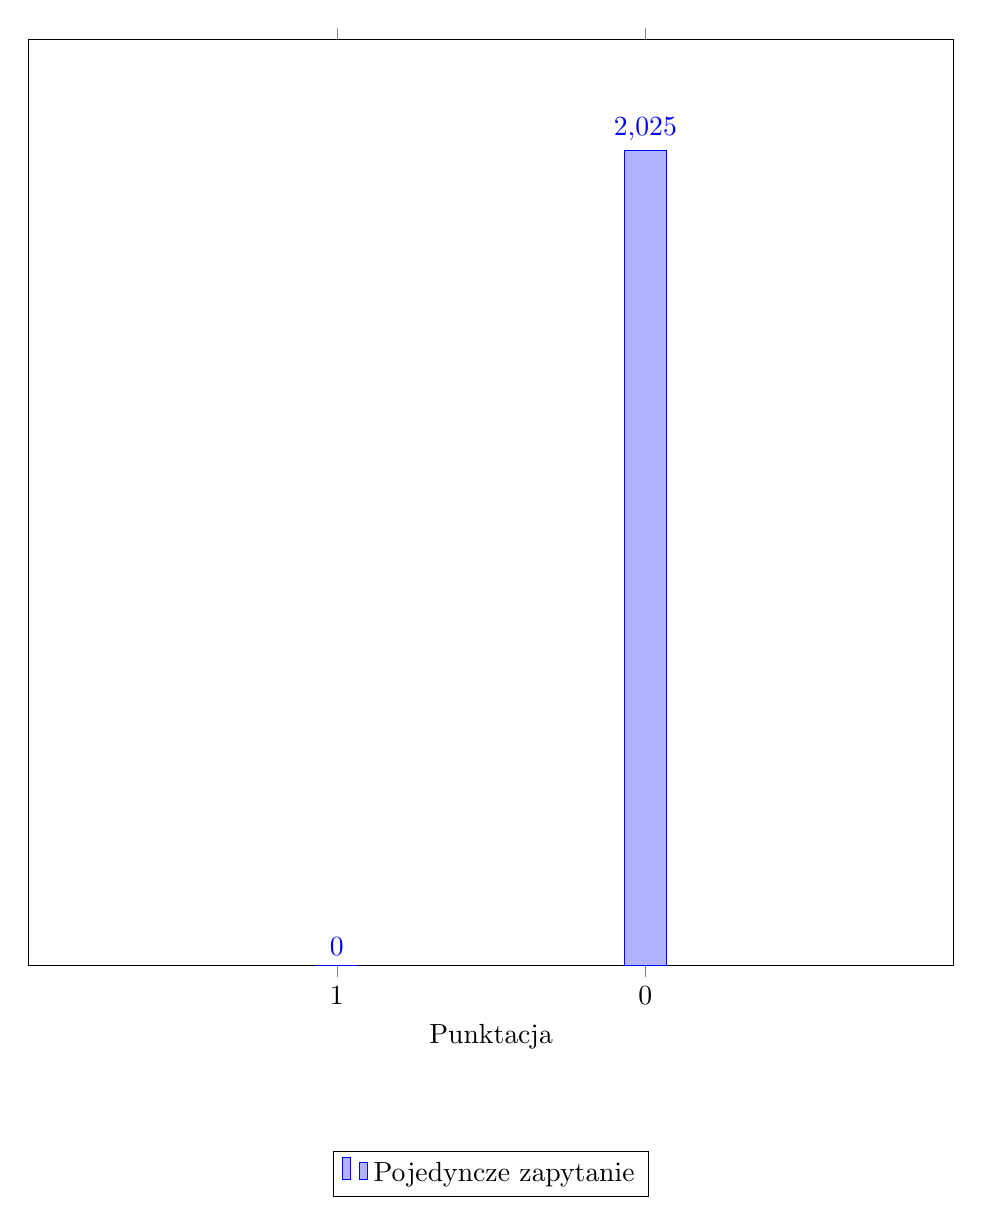
\begin{tikzpicture}
\begin{axis}[
    ybar,
    symbolic x coords={1, 0},
    xtick=data,
    %ylabel={Liczba},
    width=1.1\textwidth,
    height=1.1\textwidth,
    ytick = \empty,
    nodes near coords,
    bar width=15pt,
    enlarge x limits=1,
    ymin=0,
    ymax=2300,
    xlabel={Punktacja},
    legend style={at={(0.5,-0.20)}, anchor=north, legend columns=-1}
]
\addplot coordinates {(1,0) (0,2025)};
\addlegendentry{Pojedyncze zapytanie}
\end{axis}
\end{tikzpicture}
\end{minipage}
\caption{Wykres ocenionych wyników dla kategorii \textbf{Ograniczenia}.}
\end{figure}

W przypadku ostatniej z ocenianych kategorii, modele osiągnęły niskie oceny. Wynikało to ponownie z ogólności kategorii. Wszelkie błędy, które nie zostały wyłapane w pozostałych kategoriach, zostały rozliczone w tym miejscu. Modele  \textit{ZIMPL} straciły najwięcej punktów na tworzeniu niepotrzebnych i niezwiązanych z problemem komend. 

\begin{table}[ht]
\caption{Tabela ocenionych wyników dla kategorii \textbf{Inne wymagania}.}\label{tab:tabela22}
\centering%
\begin{tabular}{|l|c|c|}
\hline
\textbf{Punktacja} & \textbf{Generator} & \textbf{Pojedyncze zapytanie}\\
\hline
1 & 658 & 259 \\
\hline
0 & 1367 & 1766 \\
\hline
Średnia ocena & 0,32 & 0,13 \\
\hline
\end{tabular}
\end{table}


\begin{figure}[H]
\centering
\begin{minipage}{0.45\textwidth}
\centering
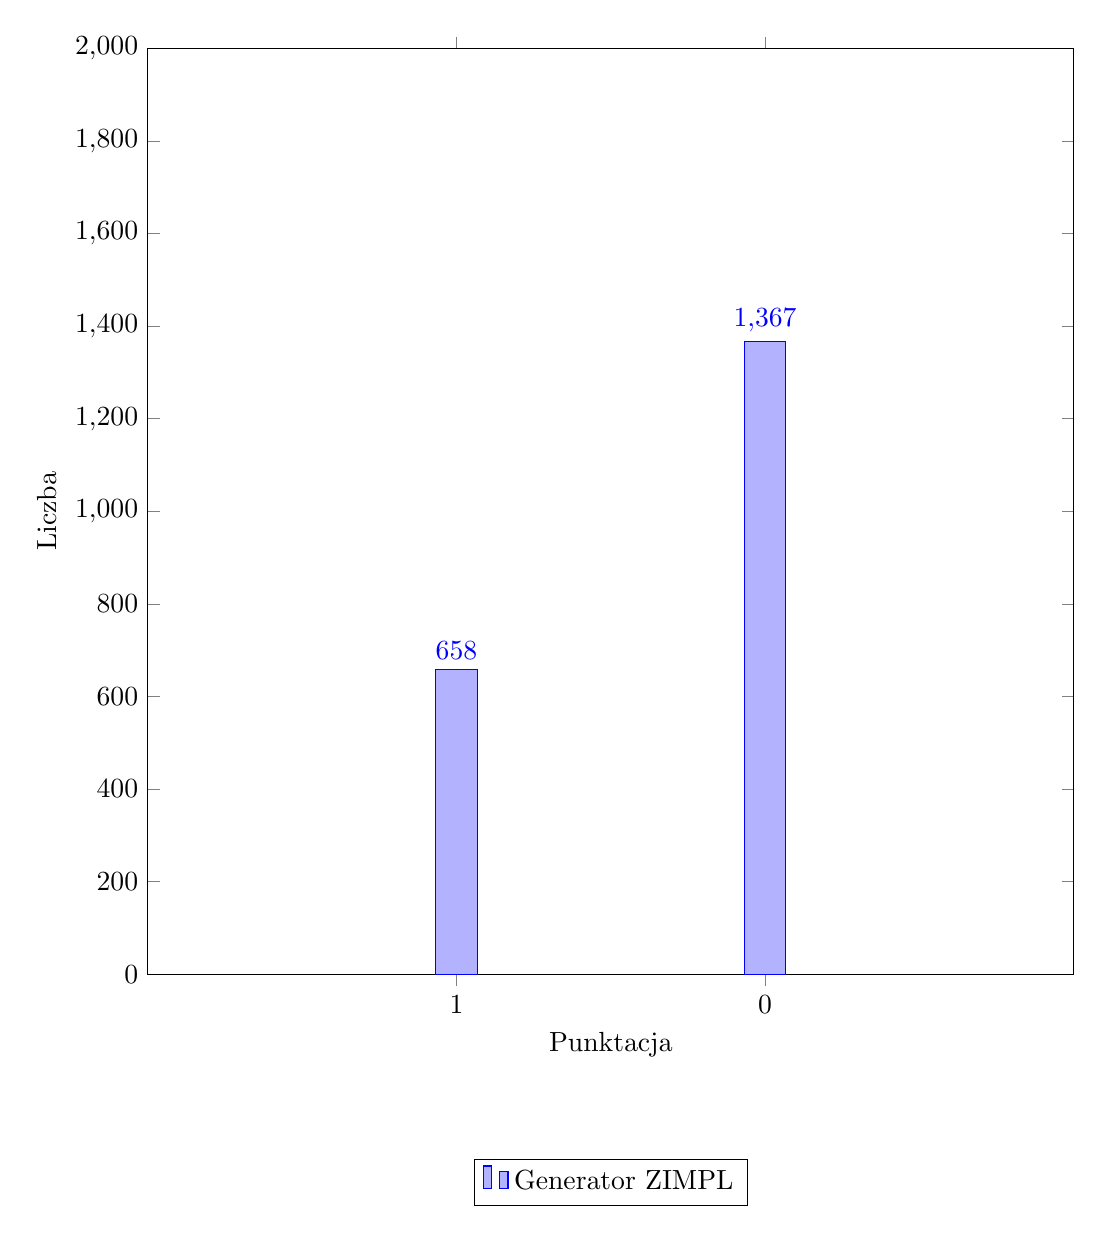
\begin{tikzpicture}
\begin{axis}[
    ybar,
    symbolic x coords={1, 0},
    xtick=data,
    ylabel={Liczba},
    width=1.1\textwidth,
    height=1.1\textwidth,
    nodes near coords,
    bar width=15pt,
    enlarge x limits=1,
    ymin=0,
    ymax=2000,
    xlabel={Punktacja},
    legend style={at={(0.5,-0.20)}, anchor=north, legend columns=-1}
]
\addplot coordinates {(1,658) (0,1367)};
\addlegendentry{Generator ZIMPL}
\end{axis}
\end{tikzpicture}
\end{minipage}%
\hspace{0.05\textwidth}
\begin{minipage}{0.45\textwidth}
\centering
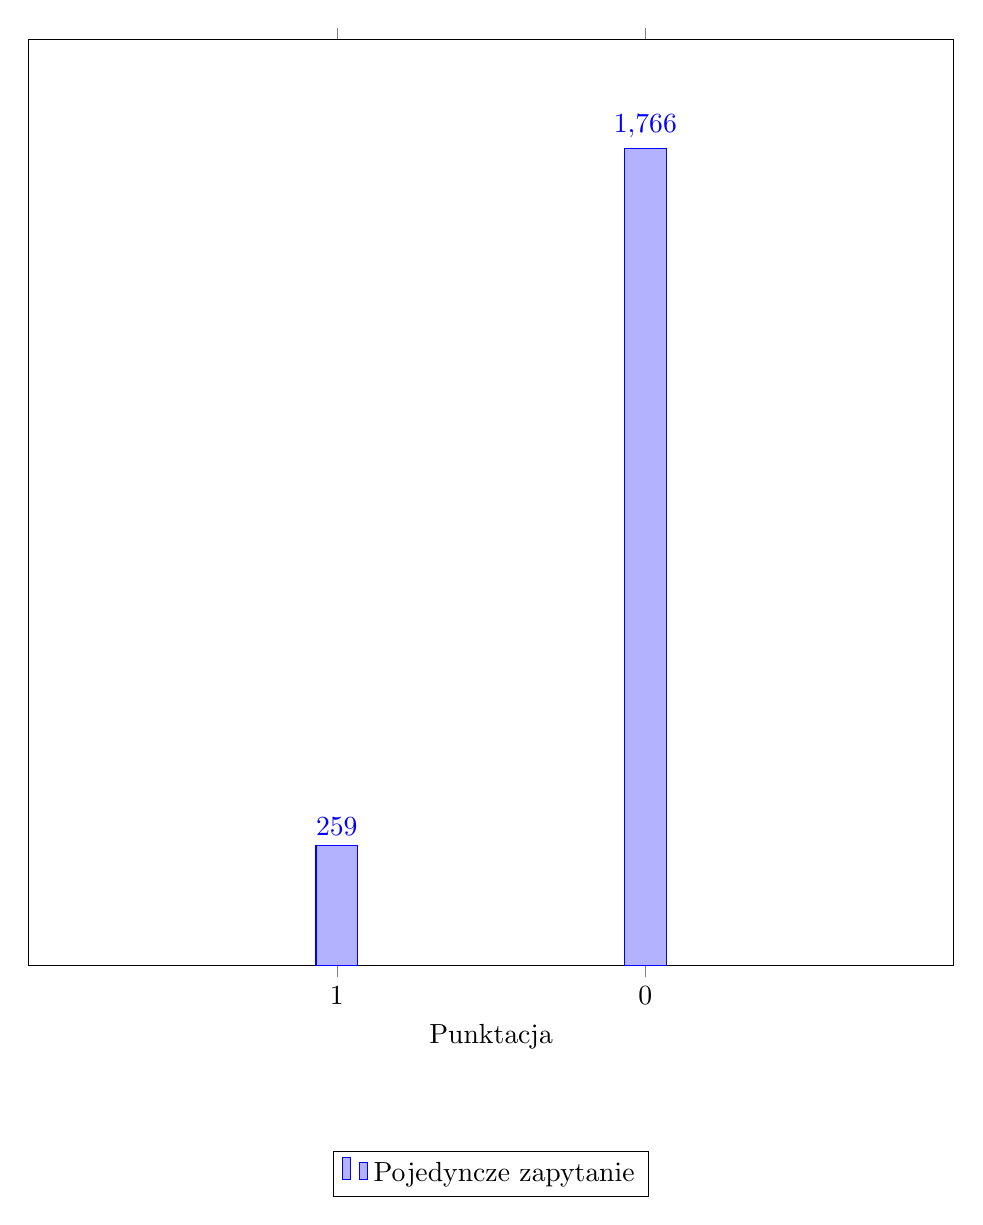
\begin{tikzpicture}
\begin{axis}[
    ybar,
    symbolic x coords={1, 0},
    xtick=data,
    %ylabel={Liczba},
    width=1.1\textwidth,
    height=1.1\textwidth,
    ytick = \empty,
    nodes near coords,
    bar width=15pt,
    enlarge x limits=1,
    ymin=0,
    ymax=2000,
    xlabel={Punktacja},
    legend style={at={(0.5,-0.20)}, anchor=north, legend columns=-1}
]
\addplot coordinates {(1,259) (0,1766)};
\addlegendentry{Pojedyncze zapytanie}
\end{axis}
\end{tikzpicture}
\end{minipage}
\caption{Wykres ocenionych wyników dla kategorii \textbf{Inne wymagania}.}
\end{figure}

W poniższym zestawieniu sumarycznych rezultatów widać, że stworzony generator kodu  \textit{ZIMPL} został znacznie lepiej oceniony, niż pojedyncze zapytanie. W większości wypadków utrzymuje on wynik w okolicy 5 punktów (średnio 4,75), co świadczy o wysokiej jakości. Ta różnica jest znacząca w porównaniu do wyniku pojedynczego zapytania, który jest niższy o 1,97 punktu utrzymując średni poziom 2,78 punktu.

\begin{table}[ht]
\caption{Tabela sumarycznej oceny wyników dla parametryzowanych modeli.}\label{tab:tabela23}
\centering%
\begin{tabular}{|l|c|c|}
\hline
\textbf{Punktacja} & \textbf{Generator} & \textbf{Pojedyncze zapytanie}\\
\hline
0 & 3 & 3 \\
\hline
1 & 1 & 80 \\
\hline
2 & 23 & 464 \\
\hline
3 & 293 & 650 \\
\hline
4 & 61 & 789 \\
\hline
5 & 1080 & 39 \\
\hline
6 & 564 & 0 \\
\hline
\textbf{Średnia ocena} & \textbf{4,75} & \textbf{2,78} \\
\hline
\end{tabular}
\end{table}

\begin{figure}[H]
\centering
\begin{minipage}{0.45\textwidth}
\centering
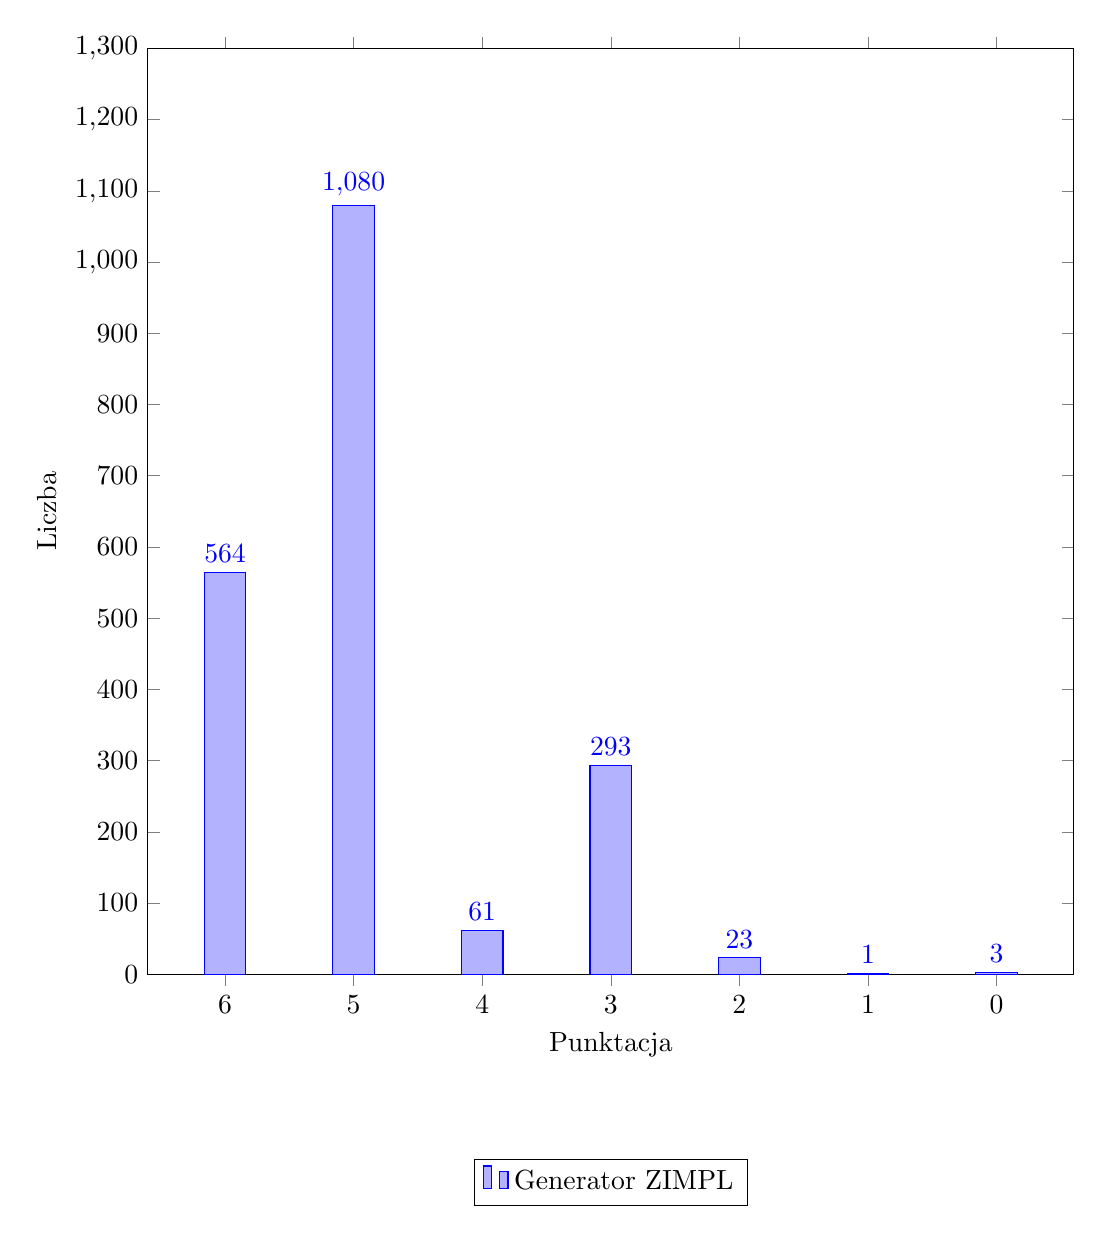
\begin{tikzpicture}
\begin{axis}[
    ybar,
    symbolic x coords={6,5,4,3,2,1,0},
    xtick=data,
    ylabel={Liczba},
    width=1.1\textwidth,
    height=1.1\textwidth,
    nodes near coords,
    bar width=15pt,
    ymin=0,
    ymax=1300,
    xlabel={Punktacja},
    legend style={at={(0.5,-0.20)}, anchor=north, legend columns=-1}
]
\addplot coordinates {(6,564) (5,1080) (4,61) (3,293) (2,23) (1,1) (0,3)};
\addlegendentry{Generator ZIMPL}
\end{axis}
\end{tikzpicture}
\end{minipage}%
\hspace{0.05\textwidth}
\begin{minipage}{0.45\textwidth}
\centering
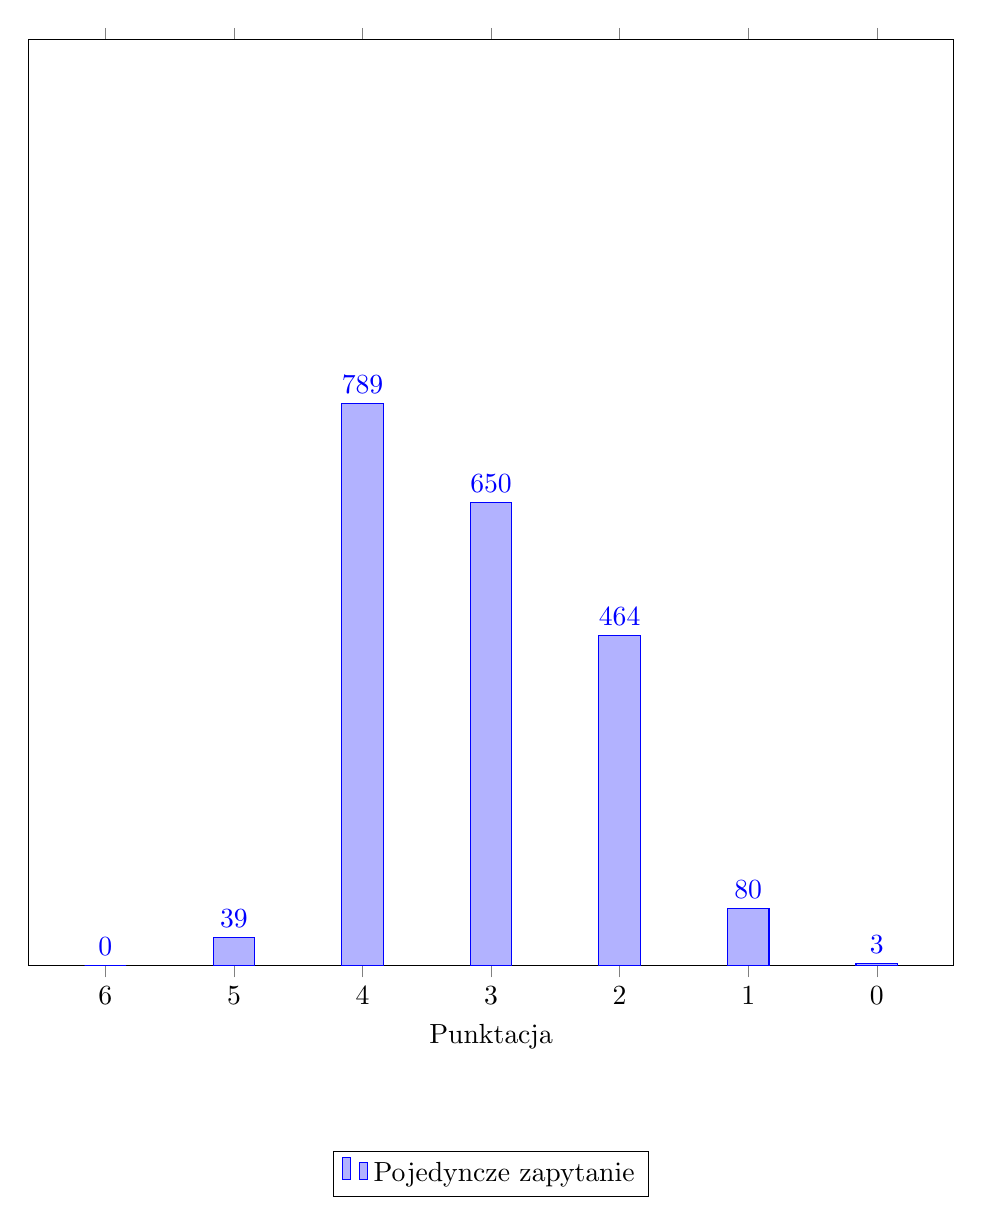
\begin{tikzpicture}
\begin{axis}[
    ybar,
    symbolic x coords={6,5,4,3,2,1,0},
    xtick=data,
    %ylabel={Liczba},
    width=1.1\textwidth,
    height=1.1\textwidth,
    ytick = \empty,
    nodes near coords,
    bar width=15pt,
    ymin=0,
    ymax=1300,
    xlabel={Punktacja},
    legend style={at={(0.5,-0.20)}, anchor=north, legend columns=-1}
]
\addplot coordinates {(6,0) (5,39) (4,789) (3,650) (2,464) (1,80) (0,3)};
\addlegendentry{Pojedyncze zapytanie}
\end{axis}
\end{tikzpicture}
\end{minipage}
\caption{Wykres prezentujący sumaryczną ocenę wyników dla parametryzowanych modeli.}
\end{figure}